% !TeX encoding = UTF-8

% 载入 SJTUThesis 模版
\documentclass[type=bachelor,lang=zh]{sjtuthesis}
% 选项
%   type=[doctor|master|bachelor],     % 可选(默认:master),论文类型
%   zihao=[-4|5],                      % 可选(默认:-4),正文字号大小
%   lang=[zh|en|de|ja],                % 可选(默认:zh),论文的主要语言
%   review,                            % 可选(默认:关闭),盲审模式
%   [twoside|oneside],                 % 可选(默认:twoside),双页或单页边距模式
%   [openright|openany],               % 可选(默认:openright),奇数页或任意页开始新章
%   math-style=[ISO|TeX],              % 可选 (默认:ISO),数学符号样式

% 论文基本配置,加载宏包等全局配置
% !TEX root = ./main.tex

\sjtusetup{
  %
  %******************************
  % 注意:
  %   1. 配置里面不要出现空行
  %   2. 不需要的配置信息可以删除
  %******************************
  %
  % 信息录入
  %
  info = {%
    %
    % 标题
    %
    zh / title           = {颗粒介质中的超声波传播},
    en / title           = {Ultrasonic Propagation in Granular Media},
    %
    % 标题页标题
    %   可使用“\\”命令手动控制换行
    %
    % zh / display-title   = {上海交通大学学位论文\\ \LaTeX{} 模板示例文档},
    % en / display-title   = {A Sample Document \\ for \LaTeX-based SJTU Thesis Template},
    %
    % 关键词
    %
    zh / keywords        = {颗粒介质, 超声波, 随机堆积},
    en / keywords        = {granular media, ultrasonic, random packing},
    %
    % 姓名
    %
    zh / author          = {何翼成},
    en / author          = {He Yicheng},
    %
    % 指导教师
    %
    zh / supervisor      = {王宇杰教授},
    en / supervisor      = {Prof. Wang Yujie},
    %
    % 副指导教师
    %
    % assoc-supervisor  = {某某教授},
    % assoc-supervisor* = {Prof. Uom Uom},
    %
    % 学号
    %
    id              = {520072910043},
    %
    % 学位
    %   本科生不需要填写
    %
    zh / degree          = {物理学学士},
    en / degree          = {Bachelor of Physics},
    %
    % 专业
    %
    zh / major           = {物理学(致远荣誉计划)},
    en / major           = {Physics (Zhiyuan Honors Program)},
    %
    % 所属院系
    %
    zh / department      = {致远学院},
    en / department      = {Zhiyuan College},
    %
    % 答辩日期
    %   使用 ISO 格式 (yyyy-mm-dd);默认为当前时间
    %
    % date                 = {2023-05-18},
    %
    % 标题页显示日期
    %   覆盖对应标题页的日期显示,原样输出
    %
    % zh / display-date    = {2023 年 5 月},
    %
    % 资助基金
    %
    % zh / fund  = {
    %                {国家 973 项目 (No. 2025CB000000)},
    %                {国家自然科学基金 (No. 81120250000)},
    %              },
    % en / fund  = {
    %                {National Basic Research Program of China (Grant No. 2025CB000000)},
    %                {National Natural Science Foundation of China (Grant No. 81120250000)},
    %              },
  },
  %
  % 风格设置
  %
  style = {%
    %
    % 论文标题页 logo 颜色 (red/blue/black)
    %
    % title-logo-color = black,
  },
  %
  % 名称设置
  %
  name = {
    % bib             = {References},
    % ack             = {谢\hspace{\ccwd}辞},
    % achv            = {攻读学位期间完成的论文},
  },
}

% 使用 BibLaTeX 处理参考文献
%   biblatex-gb7714-2015 常用选项
%     gbnamefmt=lowercase     姓名大小写由输入信息确定
%     gbpub=false             禁用出版信息缺失处理
\usepackage[backend=biber,style=gb7714-2015]{biblatex}
% 文献表字体
% \renewcommand{\bibfont}{\zihao{5}\fixedlineskip{15.6bp}}
% 文献表条目间的间距
\setlength{\bibitemsep}{0pt}
% 导入参考文献数据库
\addbibresource{refs.bib}

% 脚注格式
\usepackage[perpage,bottom,hang]{footmisc}

% 定义图片文件目录与扩展名
\graphicspath{{figures/}}
\DeclareGraphicsExtensions{.pdf,.eps,.png,.jpg,.jpeg}

% 确定浮动对象的位置,可以使用 [H],强制将浮动对象放到这里(可能效果很差)
% \usepackage{float}

% 固定宽度的表格
% \usepackage{tabularx}

% 使用三线表:toprule,midrule,bottomrule。
\usepackage{booktabs}

% 表格中支持跨行
\usepackage{multirow}

% 表格中数字按小数点对齐
\usepackage{dcolumn}
\newcolumntype{d}[1]{D{.}{.}{#1}}

% 使用长表格
\usepackage{longtable}

% 附带脚注的表格
\usepackage{threeparttable}

% 附带脚注的长表格
\usepackage{threeparttablex}

% 算法环境宏包
\usepackage[ruled,vlined,linesnumbered]{algorithm2e}
% \usepackage{algorithm, algorithmicx, algpseudocode}

% 代码环境宏包
\usepackage{listings}
\lstdefinestyle{lstStyleCode}{%
  aboveskip         = \medskipamount,
  belowskip         = \medskipamount,
  basicstyle        = \ttfamily\zihao{6},
  commentstyle      = \slshape\color{black!60},
  stringstyle       = \color{green!40!black!100},
  keywordstyle      = \bfseries\color{blue!50!black},
  extendedchars     = false,
  upquote           = true,
  tabsize           = 2,
  showstringspaces  = false,
  xleftmargin       = 1em,
  xrightmargin      = 1em,
  breaklines        = false,
  framexleftmargin  = 1em,
  framexrightmargin = 1em,
  backgroundcolor   = \color{gray!10},
  columns           = flexible,
  keepspaces        = true,
  texcl             = true,
  mathescape        = true
}
\lstnewenvironment{codeblock}[1][]{%
  \lstset{style=lstStyleCode,#1}}{}

% 直立体数学符号
\providecommand{\dd}{\mathop{}\!\mathrm{d}}
\providecommand{\ee}{\mathrm{e}}
\providecommand{\ii}{\mathrm{i}}
\providecommand{\jj}{\mathrm{j}}

% 国际单位制宏包
\usepackage{siunitx}

% 定理环境宏包
\usepackage{ntheorem}
% \usepackage{amsthm}

% 绘图宏包
\usepackage{tikz}
\usetikzlibrary{arrows.meta, shapes.geometric}

% 数据图表宏包
\usepackage{pgfplots}
\pgfplotsset{compat=newest}

% 一些文档中用到的 logo
\usepackage{hologo}
\providecommand{\XeTeX}{\hologo{XeTeX}}
\providecommand{\BibLaTeX}{\textsc{Bib}\LaTeX}

% 借用 ltxdoc 里面的几个命令方便写文档
\DeclareRobustCommand\cs[1]{\texttt{\char`\\#1}}
\providecommand\pkg[1]{{\sffamily#1}}

% hyperref 宏包在最后调用
\usepackage{hyperref}

% E-mail
\providecommand{\email}[1]{\href{mailto:#1}{\urlstyle{tt}\nolinkurl{#1}}}


\begin{document}

%TC:ignore

% 标题页
\maketitle

% 原创性声明及使用授权书
\copyrightpage
% 插入外置原创性声明及使用授权书
% 此时必须在导言区使用 \usepackage{pdfpages}
% \copyrightpage[scans/sample-copyright.pdf]

% 前置部分
\frontmatter

% 摘要
% !TEX root = ../main.tex

\begin{abstract}[zh]
  中文摘要应该将学位论文的内容要点简短明了地表达出来,应该包含论文中的基本信息,体现科研工作的核心思想。摘要内容应涉及本项科研工作的目的和意义、研究方法、研究成果、结论及意义。注意突出学位论文中具有创新性的成果和新见解的部分。摘要中不宜使用公式、化学结构式、图表和非公知公用的符号和术语,不标注引用文献编号。硕士学位论文中文摘要字数为 500 字左右,博士学位论文中文摘要字数为 800 字左右。英文摘要内容应与中文摘要内容一致。

  摘要页的下方注明本文的关键词(4 \textasciitilde{} 6个)。
\end{abstract}

\begin{abstract}[en]
  
\end{abstract}


% 目录
\tableofcontents
% 插图索引
\listoffigures*
% 表格索引
\listoftables*
% 算法索引
\listofalgorithms*

% 符号对照表
% !TEX root = ../main.tex

\begin{nomenclature*}
\label{chap:symb}

\begin{longtable}{rl}
  $d$  & 颗粒粒径 \\  
  $\phi$ & 体积分数 \\
  $\chi$ & 等效温度 \\
  $\lambda$ & 波长 \\
  $f$ & 频率 \\
  $V_{\text{T.O.F.}}$ & 飞行时间法测得的声速\\
  $p(t)$ & 时域声压\\
  $p_{i}(t)$ & 入射声压\\
  $\widetilde{Z}_{S}(\omega)$ & 角频域声阻抗\\
  $L$ & 颗粒介质厚度\\
  $t_{0}$ & 响应信号波前到达时间\\
  $t_{1}$ & 响应信号波峰到达时间\\
  $t_{2}$ & 响应信号首次过零到达时间\\
  $P$ & 单轴应力\\
  $V_{L}$ & 纵波声速\\
  $V_{T}$ & 横波声速\\
  $W$ & 首峰归一化宽度\\
  $\alpha$ & 衰减系数\\
  $V_{\varphi}$ & 相速度\\
  $C_{i,j}(\tau)$ & 信号 $i$ 和 $j$ 的互相关函数\\
  $\tau$ & 延迟时间\\
  $K$ & 体弹性模量\\
  $G$ & 剪切模量\\
  $\rho^{*}$ & 颗粒介质密度\\
  $\rho$ & 颗粒材料密度\\
  $Z$ & 颗粒平均接触数\\
  $C_{n}$ & 颗粒在法向的接触强度系数\\
  $C_{t}$ & 颗粒在切向的接触强度系数\\
  $f_{n}$ & 法向接触力\\
  $f_{t}$ & 切向接触力\\
  $w$ & 颗粒重叠量\\
  $a$ & 颗粒接触圆面半径\\
  $G_{g}$ & 颗粒材料剪切模量\\
  $\nu_{g}$ & 颗粒材料泊松比\\
  $\mathbf{I}^{(nm)}$ & 从颗粒 $m$ 指向 $n$ 的单位矢量\\
  $\Delta s$ & 颗粒间切向相对位移 \\
  $\lambda_{L}$ & 颗粒材料第一 Lamé 常数\\
  $\mu_{L}$ & 颗粒材料第二 Lamé 常数\\
  $\mathbf{e}_{ij}$ & 颗粒介质应变张量\\
  $\sigma_{ij}^{(n)}$ & 颗粒 $n$ 的 Cauchy 应力张量\\
  $\delta_{ij}$ & 克罗内克符号\\
  $C_{ijkl}^{*}$ & 颗粒介质的等效模量张量\\
  $\lambda_{L}^{*}$ &颗粒介质的等效第一 Lamé 常数\\
  $\mu_{L}^{*}$ & 颗粒介质的等效第二 Lamé 常数\\
  $P_{\text{eff}}$ & 有效应力\\
  $k(\omega)$ & 频域上的波数\\
  $\nu_{K}$ & 体弹性模量的涨落\\
  $L_{c}$ & 体弹性模量的关联长度\\

  
  $D$ & 扩散系数\\
  $\tau_{\alpha}$ & 非弹性吸收时间\\
  $\nu_{e}$ & 能量传输速度\\
  $U_{0}$ & 声源能量\\
  $l^{*}$ & 平均自由程\\
  $Q$ & 品质因子\\
  $G_{g}$ & 颗粒材料剪切模量\\
  $\mu_{f}$ & 颗粒间摩擦系数\\
  $u_{t}$ & 切向振幅\\
  $u_{n}$ & 法向振幅\\
  $\mu$ & 介质切变黏度\\
  $\mu_{B}$ & 介质体变黏度\\
  $\kappa$ & 介质热导率\\
  $c_{v}$ & 定容热容\\
  $c_{p}$ & 定压热容\\
  $\beta$ & 介质的非线性系数\\
  $\rho_{0}$ & 介质在平衡态下的密度\\
  $c_{0}$ & 介质在平衡态下的声速\\
  $\xi(a)$ & 相对物质坐标 $a$ 的流体粒子位移量\\
  $u_{n\omega}$ & $n$ 倍频谐波分量\\
  $\alpha_{\mu}$ & 黏性吸收系数\\
  $\alpha_{h}$ & 热吸收系数\\
  $\omega$ & 角频率\\
  $\Psi_{i,j}(\tau)$ & 信号 $i$ 和 $j$ 的归一化交叉关联函数\\
  $\beta_{\text{Hertz}}$ & Hertz 接触力一阶非线性系数\\
  $\delta_{\text{Hertz}}$ & Hertz 接触力二阶非线性系数\\
  $u_{t}^{E}(f_{t})$ & 切向振幅的弹性响应分量\\
  $u_{t}^{H}(f_{t})$ & 切向振幅的耗散响应分量\\
  $D_{n}$ & 法向接触力的刚度系数\\
  $D_{t}$ & 切向接触力的刚度系数\\
  $f_{t}^{*}$ & 切向接触力的幅值\\

  $\varepsilon_{\text{pl}}$ & 塑性形变量\\
  $V_{f}$ & 颗粒介质的自由体积\\
  $n_{\pm}$ & 处于状态 $\pm$ 的数密度\\
  $\sigma$ & 介质所受的偏应力\\
  $n_{\infty}$ & $(n_{-} + n_{+})$ 在稳定平衡态下的值\\

\end{longtable}

\end{nomenclature*}


%TC:endignore

% 主体部分
\mainmatter

% 正文内容
% !TEX root = ../main.tex

\chapter{绪论}

\section{颗粒物质}

“当一个物体被分作几个单独运动的小部分时,它是液态的;而当它的所有部分都接触在一起时,它是固态的。” 这就是 17 世纪笛卡尔对于颗粒物质机械性质的朴素认知。颗粒物质在自然界中广泛存在,拥有类似于寻常物质的固(颗粒静堆积,也被称作 jammed state,即阻塞态)、液(颗粒流,也被称作 unjammed state,即非阻塞态)、气(颗粒分布均匀、快速运动)三态\cite{RevModPhys.68.1259},其共通特征是由离散物质构成的聚集系统,如沙漠、土壤、泥石流、沙尘暴;而在人类文明中,颗粒物质无疑也占有重要地位,如谷物堆积、矿石输运、药物粉末等生产行为,其背后也隐藏着颗粒堆积与流变的学问。即使是成本相对低廉的的煤炭、水泥、沙砾等工业材料,总共的生产与加工对地球上生产能源消耗的比例也来到了约 \num{10}\%\cite{duran2000sands}。因此对于颗粒物质的研究与理解,不仅有益于进一步认知自然界,从而防治地震、滑坡、雾霾、沙漠化等自然灾害,还有助于减少工业中的能源损失,进而提升人类工业文明的生产效率、提高生产质量。

颗粒物质的物理学是一门复杂的学科。颗粒物质通常被定义为尺度大于微米量级的宏观离散体,通过接触、碰撞等形式聚集组成的多体系统。颗粒物质拥有着丰富的物理特性,总结如下:

\begin{enumerate}
  \item 宏观性。足够的尺度与质量使得颗粒介质的运动无需考虑分子层面的热运动以及量子层面的概率分布效应,一种常见的分析思路是计算对比热力学尺度的 $k_{B}T$ 与颗粒尺度对应的引力势能 $mgd$,而常温($\sim$ 300 \unit{\kelvin})外部激励对于颗粒堆积的作用可以忽略(目前也的确存在对沙堆进行循环热剪切的相关实验\cite{YIN2023100503},但是这与我们论证不能通过温度遍历相空间的思路显然不同)。对于颗粒物理的力学研究也大多基于经典的牛顿力学;
  \item 离散性。在以等半径硬球组成的颗粒固体中,颗粒通常以随机的方式形成堆积,即介质中通常存在着空隙;对应地,使用体积分数 $\phi$ 来评估颗粒介质的空间利用率,其中对于等大硬球的情形存在着随机松散堆积(random loose packing,RLP)和随机密堆积(random close packing)两个体积分数极限,分别约为 0.55\cite{PhysRevLett.64.2727} 和 0.64\cite{RevModPhys.82.789}。随机性堆积的非晶结构使得传统的连续介质力学对颗粒介质的描述存在偏差\cite{RevModPhys.71.435};
  \item 多体性。三体问题已经是能产生混沌现象的复杂力学体系;即使只是静止状态下的颗粒固体,对于 $N$ 个颗粒进行描述也仍然需要多达 $3N$ 个正则坐标,即颗粒介质的多体特征使得其具有难以求解的极高自由度,所以对其进行宏观力学上的建模求解也是困难重重;
  \item 耗散性。颗粒间复杂的相互摩擦与碰撞使得系统中的各成员能迅速将动能转化为分子层面的热运动。因此颗粒系统中存在强耗散性,在失去外部能量驱动的情况下可以长期处于某一亚稳态(metastable state)。常规的统计力学假设,即系统在温度激励下可以遍历相空间中的微观态,对于颗粒介质而言失效。换言之,颗粒介质是典型的非平衡态系统;
  \item 敏感性。颗粒介质中存在高度复杂的力链与接触网络,而振动、剪切等外部激励容易使得颗粒进行重排(Rearrangement),使得这两种网络都具有高敏感性。因此对颗粒物质展开实验研究时,需要慎重考虑过程中的技术细节,避免观测手段本身对颗粒介质造成的扰动介入到所观察的实验现象中。
  \item 多分散性(polydispersity)。该术语原意是描述高分子聚合物的分子量不均一性,被援引至颗粒介质中用于指代多种不同颗粒的混合。虽然在大多数实验与理论中都是使用等大硬球模型来描述颗粒介质,但是在真实世界中的颗粒介质中,颗粒的尺寸、形状\cite{vandenwildenbergProbingEffectParticle2015}、材料等参数不只是非均匀的,而且其在各自参数定义域上的分布也未必有规律,同时伴随着相分离\cite{doi:10.1126/sciadv.abe8737}等复杂动力学现象。
\end{enumerate}

颗粒物质的物理学也是年轻的学科。2005 年 Science 提出的 125 个最重要前沿科学问题\cite{doi:10.1126/science.309.5731.78b}中,“能否发展关于湍流动力学和颗粒材料运动学的综合理论?”赫然在列;而 2021 年提出的 “新 125 个科学问题”\cite{sanders2021125}中,“集体运动的基本原理是什么?”仍然彰显着颗粒物质物理学的神秘与活力。

\section{颗粒物质的研究方法现状}


\subsection{实验方法}

针对颗粒物理中丰富的物理性质,目前已开发出多角度的实验研究方法。

\begin{enumerate}
  \item 光-弹性实验\cite{photoelasticimetry}。对于光学透明的介质,其内部应变时会展现出双折射现象,因此可以直观体现颗粒介质在受单轴剪切、环形剪切等外部作用下其内部的应力分布情形。但是由于偏振光在异质性介质中的传播、三维介质中的精确测量困难等问题\cite{Non-Destructive_3D_Photoelasticity},光弹性方法通常只适用于二维平面的颗粒介质;
  \item X 射线计算机断层扫描成像(computed tomography,CT)\cite{PhysRevE.68.020301}。X 射线扫描图像经由去边界、分水岭算法分割等处理后可以重构出颗粒介质的三维空间结构,从而研究颗粒介质中的接触结构与运动关系。但是该方法通常难以应用于实地实验。CT 设备本身成本已经较为昂贵,并且即使只是拍摄单张图像,其所需的存储空间也已较大(对于图像分辨率 $1021\times 1021 \times 886$,约占 $1.7\unit{\giga\byte}$ 的储存空间),因此如果对实际测量时所拍摄的多帧图像进行数据处理,还需要配备价格不菲的高性能计算资源,进一步提高了其技术门槛。CT 设备由于射线源和探测板等性能限制,因此其空间分辨精度也会存在上限。这一点对于所研究颗粒的半径(为了得到图像中清晰的颗粒边界,一般要求颗粒的直径大于 $2\unit{\milli\meter}$)、材料(金属颗粒对 X 光吸收率过高而影响成像效果,因此不能被用于辐照)都存在一定限制。除此之外,一般的 X 光成像方法都是通过射线源和接收器对受辐照的物体进行旋转扫描以进行建模,这个拍摄过程通常会长达数十秒,所以对于高时间分辨需求的情境下,X 射线方法扫描建模方法不得不使用多源同步\cite{wang2008ultrafast}的方式间接提高时间分辨率;
  \item 核磁共振\cite{CLARKE2023}。另一类对颗粒介质进行成像研究的手段,只是“光源”换为了磁场。相应的,颗粒介质中需要对应的标记原子(这种原子核需要存在非零净磁矩,如最常用的质子成像就是利用的 H$^{1}$ 核),搭建对应的磁场线圈等也存在一定的技术门槛。
\end{enumerate}

以及本文所着眼的超声波探测技术。超声波在小振幅时具有非侵入式的探测作用,在有限振幅时则对颗粒介质具有诱导重排\cite{PhysRevE.84.020301}、流化/塑性软化(elastic weakening)\cite{PhysRevE.84.020301}等泵浦(pumping)作用。因此在设计超声波探测实验时,需要考虑其振幅、频率等参数与颗粒介质的相性。

超声波探测技术根据其探测方法可以大致分为两类:

\begin{enumerate}
  \item 主动探测。超声波在颗粒介质中的传播是对其内部应力与接触结构的直接体现\cite{PhysRevB.48.15646,Jia1999UltrasoundPI,Transitional}。超声波主动探测具有非侵入性、高灵敏度等优点;真实世界中的颗粒材料通常光学不透明或者剧烈光散射,使得超声波成为颗粒物质研究中独一无二的探针。对经由颗粒介质传播后的声信号进行频谱、波形、声速、衰减、相似性参数等分析,有助于研究颗粒介质内部的结构/应力特征;
  \item 被动探测。颗粒介质受剪切等外部激励时出现应力-应变曲线,这种宏观事件伴随着内部颗粒的重排、碰撞与摩擦等介观过程,这类机械过程会激发颗粒的机械振动,即发射出携带事件信息的声信号。这种事件被称为声发射(Acoustic Emission,AE)。通过分析 AE 信号的频谱、能量、波形、振动模密度等特征\cite{PhysRevLett.120.218003,10.1029/2023JB026612,doi:10.1073/pnas.2305134120},可以对颗粒介质受应力时的蠕变(creeping)、滞滑(stick-slip)事件等特征过程进行研究。
\end{enumerate}

声学探测的时间尺度相较于成像方法的小很多,在时间分辨率这一方面存在着天然的优势\cite{PhysRevE.84.020301},因此可以被设计用于剪切带探测\cite{PhysRevE.85.051302}等连续过程实验。


\subsection{理论方法}

虽然颗粒物质是典型的非平衡态系统,但是对其进行统计力学上的描述仍在争取中。在实验中已经发现,通过如图~\eqref{fig:apparatus_of_granular} 所示的振台振动、剪切盒循环剪切等外部激励方式操纵的颗粒堆积,其存在可重复的微观态;若进一步采取等概率假设,即相同体积颗粒堆积的微观结构概率相同,那么就可以将体积 $V$ 替代传统的统计力学中的哈密顿量 $H$,从而建立适用于颗粒物质的统计力学框架。Edwards 以这种思想提出了“等效温度”的定义\cite{EDWARDS19891080}:

\begin{figure}[!hbtp]
  \centering
  \bisubcaptionbox{控制加速度 $a$ 的振台装置}{Tapping experiment setup controlling the acceleration $a$}%
                [7cm]{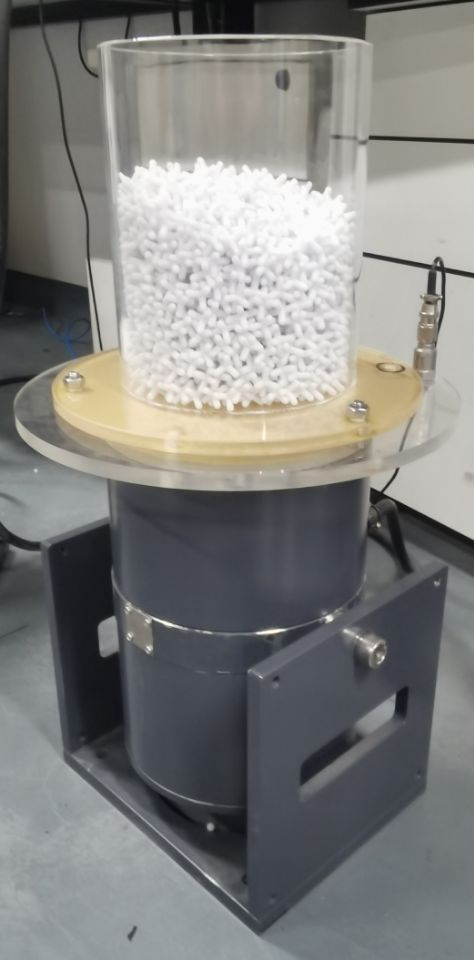
\includegraphics[height=6cm]{figures/1_tapping.jpg}}
  \hspace{1cm}
  \bisubcaptionbox{通过步进电机控制的剪切盒装置}{Shear box apparatus controlled by stepping motor}%
                [7cm]{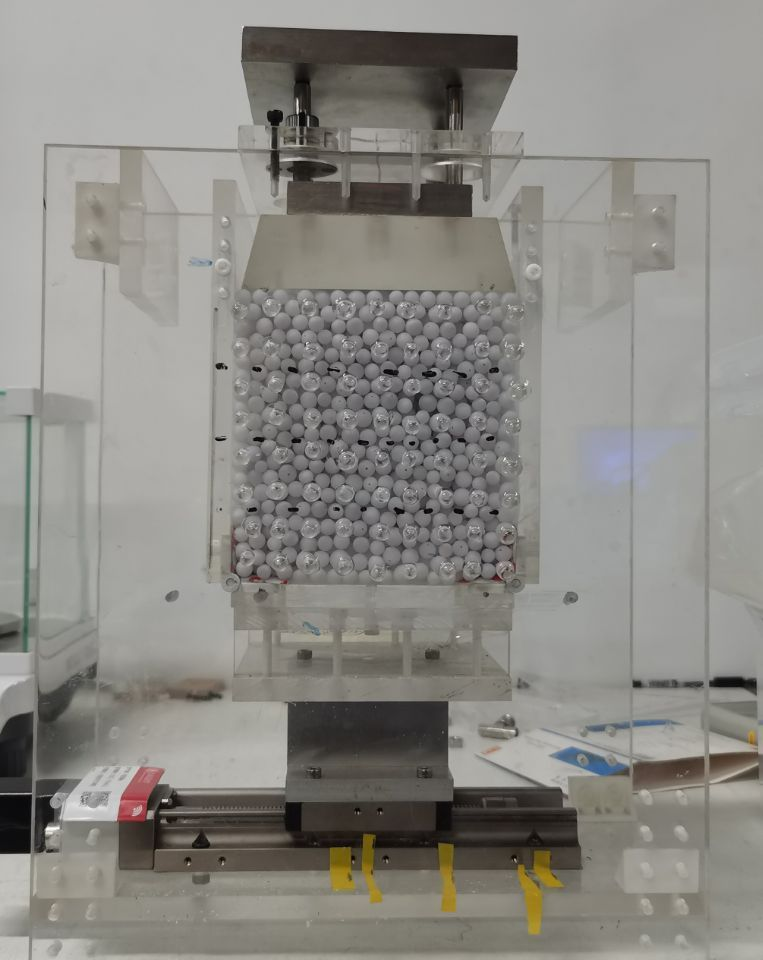
\includegraphics[height=6cm]{figures/1_shearing.jpg}}
  \bicaption{振台振动、剪切盒循环剪切等外部激励方式的装置示意图}{Schematic of the apparatus for external excitation methods such as tapping, cyclic shearing by the shear box, etc.}
  \label{fig:apparatus_of_granular}
\end{figure}

\begin{equation}
  \frac{1}{\chi} = \frac{\partial S(V)}{\partial V} = \frac{\partial \lambda\ln{\Omega(V)}}{\partial V},
\end{equation}

其中 $\chi$ 为等效温度(正式变量名为 Compactivity),$S$ 为熵,$\Omega(V)$ 是给定堆积体积 $V$ 下的微观态数目,$\lambda$ 是类比玻尔兹曼常数 $k_{B}$ 的常数。已有实验证明,这种定义的等效温度与通过涨落耗散效应定义的温度具有一致性\cite{PhysRevLett.129.228004}。

对于声学而言,在理论上依靠的主要是非线性声学\cite{10.1029/93JB02974}、等效介质理论(Effective Media Theory,EMT)\cite{WALTON1987213},依托于辐射传递方程(Radiative Transfer Equation,RTE)的扩散行为近似\cite{PhysRevLett.93.154303,PhysRevApplied.16.034009}。

\begin{figure}[!htp]
  \centering
  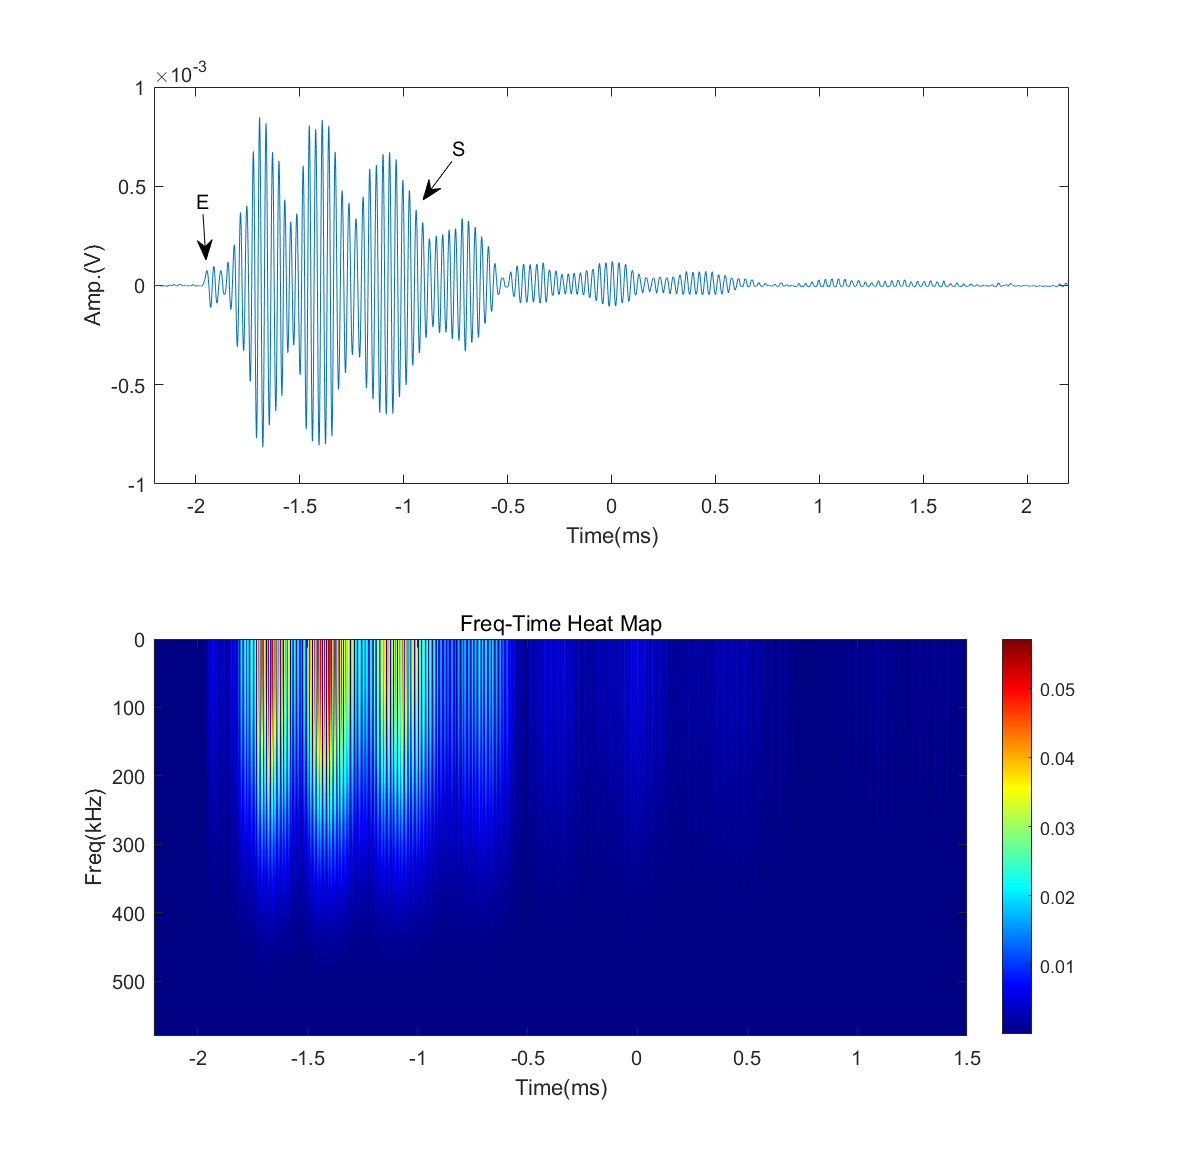
\includegraphics[height=10cm]{figures/1_heat_map.png}
  \bicaption{颗粒介质中典型的声信号。由相干首波(E)和散射尾波(S)组成。下图展示了声信号在时域上的各频率分量强度。}{Typical acoustic signal in granular media. It consists of a coherent first wave (E) and a scattering tail wave (S). The following figure illustrates the intensity of each frequency component in the acoustic signal along the time domain.}
  \label{fig:acoustic_signal}
\end{figure}

图~\ref{fig:acoustic_signal} 展示了超声波在颗粒固体中传播的示意图。可以观察到,超声波通常由相干首波(Coherent Wave,简略为 E)与散射尾波(Codalike Scatter Wave,简略为 S)。 相干波是由颗粒介质中复杂力链自平均形成的,因此对应力与接触构型不敏感,而散射波则是对接触构型非常敏感,这一点与相干波完全相反\cite{PhysRevLett.93.154303}。

在连续介质力学中我们已经知道,三维介质中的波传播分为两种模式,即纵波/压缩波(Longitudinal Wave/Compressional Wave),以及横波/剪切波(Transverse Wave/Shear Wave)。这两种模式波引入到颗粒介质中时,即分别对应了其宏观统计性质的体弹性模量 $K$ 与剪切模量 $G$。EMT 理论综合了颗粒介质特有的体积分数 $\phi$、平均接触数/配位数 $Z$ 等物理量以及连续介质力学中的弹性模量,从而预测颗粒介质中不同模式的声速等物理量。

声学对于颗粒介质的研究范式大致可以根据等效波长 $\lambda_{\text{eff}} = V_{\text{eff}}/f_{c}$ 与振幅 $A$ 来进行总结分类。为方便我们记颗粒直径尺度为 $d$。

\begin{itemize}
  \item $\lambda_{E}\gg d$。此时关心的是在颗粒介质中的相干弹性波(coherent elastic waves)。由于此时颗粒介质的力学响应可以类比于寻常固体,所以 EMT 采用仿射变换近似(affine approximation)、平均场近似等方法将其处理为等效的连续介质。此时关心的是通常是横纵波速 $V_{P}$、$V_{S}$ 与等效介质弹性模量 $K$、$G$ 之间存在的关系。
  \item $\lambda_{E}\sim d$。此时声波在颗粒介质中的传播表现出强烈的多重散射特征。颗粒接触点的耗散性使得声波在颗粒介质中的衰减吸收大大加强了,因此研究者提出了扩散行为近似\cite{PhysRevLett.93.154303}、非线性波方程\cite{Transitional,hamilton_nonlinear_1998}等模型来对颗粒介质进行研究。在这些模型中,品质因子 $Q$、平均自由程 $l^{*}$ 等参数用于研究颗粒因接触点等因素产生的耗散性。
  \item $A\rightarrow 0$。对于小振幅声波,颗粒介质的非线性仅体现为其等效黏度 $\eta$ 等介质固有特征,且不会对颗粒介质的接触与应力结构造成显著影响。在此范围内我们将超声波视为非侵入性探针;
  \item $A\rightarrow \delta$。对于有限振幅声源,颗粒介质的非线性将被进一步激发,其等效黏度将会根据超声波振幅而产生变化,即声源激励已经对颗粒介质造成泵浦效果。比如利用超声波诱导倾斜面上的颗粒介质发生滑坡(landslide,avalanche)\cite{PhysRevE.102.042901},以及地震波诱导相邻地震成核(earthquake nucleation)区域的二次地震(co-seismic)\cite{Johnson_2005}等现象。
\end{itemize}

在本文中将使用激发与接收压缩波的成对声学探头,探究在不同应力和厚度下等大硬球颗粒介质对于超声波的响应情况,从而理解颗粒介质的内部结构与力学特性。

\section{本章小结}

本章介绍了颗粒物质的基本定义和丰富特性,以及目前在颗粒物理领域常见的实验和理论方法。在阐述了一般的声学研究范式后,我们将在以下的章节中详细展开相关实验,从而理解颗粒介质对于超声波的非线性响应。
% !TEX root = ../main.tex

\chapter{相干首波}

\section{声速的测量}

任何合格的物理本科生都熟悉如何在空气或水中测量声速,如共振波节法、相位法、时差法。前两者的原理都是寻找固定频率信号的某个特殊相位(如峰值所对应的 $\uppi/2 + 2n\uppi$,$n\in\mathbb{Z}$)下的空间位置,从而通过逐差法确定声波的波长;后者则是考虑到了声学探头中压电陶瓷进行声-电转换所需要的固有时间,因此通过拟合空间位置与到达时间的斜率以确定声速。事实上,在颗粒固体中测量声速时,上述方法都有不同程度的应用,如 Paul A.Johnson 和 Xiaoping Jia 同时使用共振法与行波法(即飞行时间法,Time of Flight, T.O.F.)测定颗粒介质中的声速\cite{Johnson_2005};而在地震学中,基于连续小波变换(Continuous Wavelet Transform, CWT)和频散能量图求解地震波相速度的方法也被广泛应用。本节将介绍如何使用飞行时间法与频散能量图测量颗粒介质中的声速。

\subsection{装置搭建}

目前部署的声学探测与激励系统部件如下:

\begin{itemize}
  \item Tektronix Arbitrary Function Generator AFG31021。该仪器可以按照实验需求产生如连续正弦波、某循环数正弦波列、单频脉冲等电压信号,用于激励声学探头产生对应机械振动。其支持写入自定义函数来对信号波形进行控制;
  \item Tektronix TBS2204B 示波器。该示波器通过 BNC 接口对多达 $4$ 个独立模拟电压信号进行同步采集,可用于记录试探信号与在颗粒介质中传播后的响应信号。示波器的采样率最高可达 $1\unit{\giga\hertz}$,单次采样长度最高可达 $5\times 10^{6}$。通过 IPv4 网口可使用 TekScope 软件对 TBS2204B 进行数据读取和记录,并且进行简单程度的操控(开始/停止记录)等;
  \item ATA-101B Power Amplifier。可以设置输入与输出的线缆阻抗(目前声学常用线缆都是 $50\unit{\ohm}$),其主要功能是以最小步长 $2\unit{\decibel}$ 放大 AFG31021 产生的电压信号,从而使声学探头产生更高需求的声压振幅,通常适用于有限振幅波传播的非线性等实验中。可设定的最大放大效果为 $20\unit{\decibel}$,但是由于其固有的频域放大极限,如果初始输入的电压信号幅值已经较大,未必能完全做到这一点;
  \item 清诚声发射 G150 与 W800 (成对)声学探头。声学探头在相关领域中又被称为换能器(Transducer),即压电陶瓷既能够将射频线缆传输的模拟电压信号通过电-压效应转换为机械振动(声信号),又能够通过监测机械振动、通过压-电效应转换为模拟电压信号,从而进行进一步的信号处理与分析。G150 和 W800 分别是适用于 $60-400\unit{\kilo\Hz}$ 和 $50-800\unit{\kilo\hertz}$ 频域范围内工作的探头型号,应当根据实验需求选取合适的一对探头。两个型号的声学探头主体都是 $\varphi 19\unit{\milli\meter}\times 15\unit{\milli\meter}$ 的圆柱体,因此便于安装于同一颗粒容器中;
  \item 单轴应力圆柱容器。通过 SOLIDWORKS 软件设计并采用亚克力板制作的容器(采用透明容器是为了兼容未来可能的 X 射线扫描建模需求)。容器内径为 $D = 90\unit{\milli\meter}$, 最高支持厚度为 $13\unit{\centi\meter}$ 的颗粒介质进行实验。设置四轴活塞对容器内的颗粒介质施加单轴应力,活塞与容器底部中心均留有 $\varphi 19\unit{\milli\meter}$ 的孔洞用于安装声学探头。容器壁通过 $10\unit{\milli\meter}$ 的亚克力板弯曲为圆筒制作,因此可以承担实验需求范围的应力。探头和容器均未考虑防水/密封处理。
\end{itemize}

%%% 这里放实验装置部件的示意图

%%% 找到一个用 tikz 画工作流示意图的方法

需要说明的是,一般情况下作用于接收器表面的声压 $p(t)$ 都并不等于入射波的声压 $p_{i}(t)$,这是由探头的声阻抗 $\widetilde{Z}_{S}(\omega)$ 导致的:

\begin{equation}
  p(t) = \left(1 + \frac{\widetilde{Z}_{S}(\omega)}{\rho_{0}c_{0}S}\right) =\widetilde{K}(\omega)p_{i}(t).
\end{equation}

其中 $\rho_{0}$ 与 $c_{0}$ 是介质中平衡态下的密度和声速,$S$ 是圆面探测器的面积。接收声压 $p(t)$ 通过非幺正角频率傅里叶变换得到的频谱为

\begin{equation}
  F(\omega) = \int_{-\infty}^{+\infty}\widetilde{K}(\omega)p_{i}(t){\ee}^{-\ii\omega t}\mathrm{d}t = \widetilde{K}(\omega)F_{i}(\omega).
\end{equation}

其中 $F_{i}(\omega)$ 为入射波声压的非幺正角频率傅里叶变换。因此入射波声压 $p_{i}(t)$ 为

\begin{equation}
  p_{i}(t) = \frac{1}{2\uppi}\int_{-\infty}^{+\infty}\frac{F(\omega)}{\widetilde{K}(\omega)}{\ee}^{\ii\omega t}\mathrm{d}\omega\label{eq:response_correct}
\end{equation}

在实验中,由于我们使用的是一对同工作频域的探头,面对面接触时可以简单视为声波经历了两次同样的声阻抗过程,且假定压电效应呈现线性($p\propto U$)。那么,我们可以设定信号发生器产生的电压信号为 $U_{0}(\omega)$,则接收到的电压信号为

\begin{equation}
  U(\omega) = \widetilde{K}(\omega)^{2}U_{0}(\omega).
\end{equation}

图~\ref{fig:response_factor} 展示了设定源信号为一系列相同振幅、不同频率 $\omega_{n}$ 的连续正弦波列 $\{U(\omega_{n})\}$ 时测定的探头响应系数 $\widetilde{K}(\omega)$。

\begin{figure}[!htp]
  \centering
  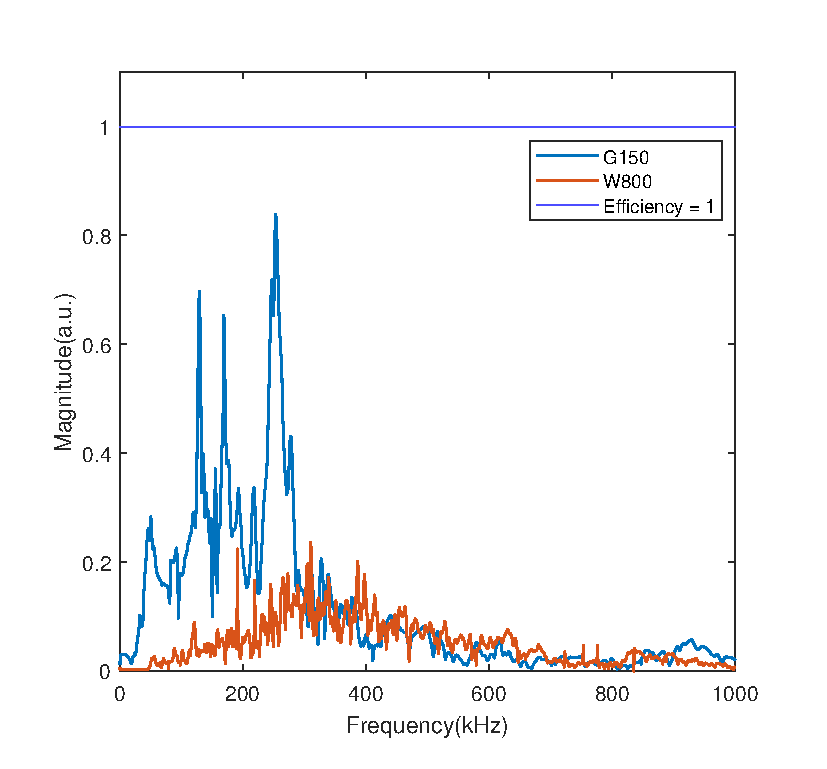
\includegraphics[height=8cm]{2_response_factor.eps}
  \bicaption{G150 与 W800 两种声学探头响应系数 $\widetilde{K}(\omega)$}{Response factor $\widetilde{K}(\omega)$ of G150 and W800 acoustic sensors}
  \label{fig:response_factor}
\end{figure}

观察可知,G150 在 \numrange{60}{400}\unit{\kilo\hertz} 频域内的响应系数非常接近 $1$, 而超出其工作频域的响应系数迅速跌落;而 W800 在我们关心的频域 \numrange{0}{1000}\unit{\kilo\hertz} 内虽然响应系数均不高,但是胜在响应曲线相对平稳。因此在实验时,如果信号集中于超声频域内的较低成分,那么选择 G150 将是更合理的;在关心较广的频域下的声学参数(比如衰减、相速度等)时,W800 的性能相对优异。为了弥补 W800 本身响应系数较低的缺陷,未来可以考虑使用 Physics of Acoustic Company 的 2/4/6 Type 等前置放大器来对有效信号进行增强。

我们后续实验便可以借助式~\eqref{eq:response_correct} 来对实验中采集的响应信号进行修正,这对幅值相关的声学测量实验意义重大。

\subsection{飞行时间法测定颗粒介质中的声速}

飞行时间法测定声速的原理即测量试探声波从声源探头到接收探头的时间差 $\Delta t$,从而计算得到

\begin{equation}
  V_{\text{T.O.F.}} = \frac{L}{\Delta t}.
\end{equation}

其中 $L$ 是颗粒介质的厚度。但是如何准确定义声波的到达时间(Arrival Time)是值得商榷的问题。Ellák Somfai 等人定义颗粒介质中声波的三种不同的到达时间:波前到达时间 $t_{0}$(由于噪声的存在,波前通常被定义为上升沿峰值 $A_{1}$ 的 $\num{10}\%$ 处,部分更激进的研究者会选取为 $3\%$),波峰到达时间 $t_{1}$,首次过零时间 $t_{2}$\cite{PhysRevE.72.021301}。良好定义的波速应当满足在不同厚度下测得的结果相近,因此我们可以按照其确定在使用飞行时间法测定声速时的最佳信号参考点。

%%% 这里放参考文献的三个不同到达时间的示意图

\subsubsection{信号最佳参考点选取}

我们在实验中使用 Tektronix 示波器对源信号与响应信号进行了同步采集,因此容易确定具体的时间起点。基于调整噪声阈值、最小半高宽等参数的寻峰算法,我们可以准确定位源信号的峰值,从而根据因果关系筛去可能错误识别的噪声。图~\ref{fig:reference_point}是对典型的响应信号进行三种不同到达时间识别的实例。


\begin{figure}[!htp]
  \centering
  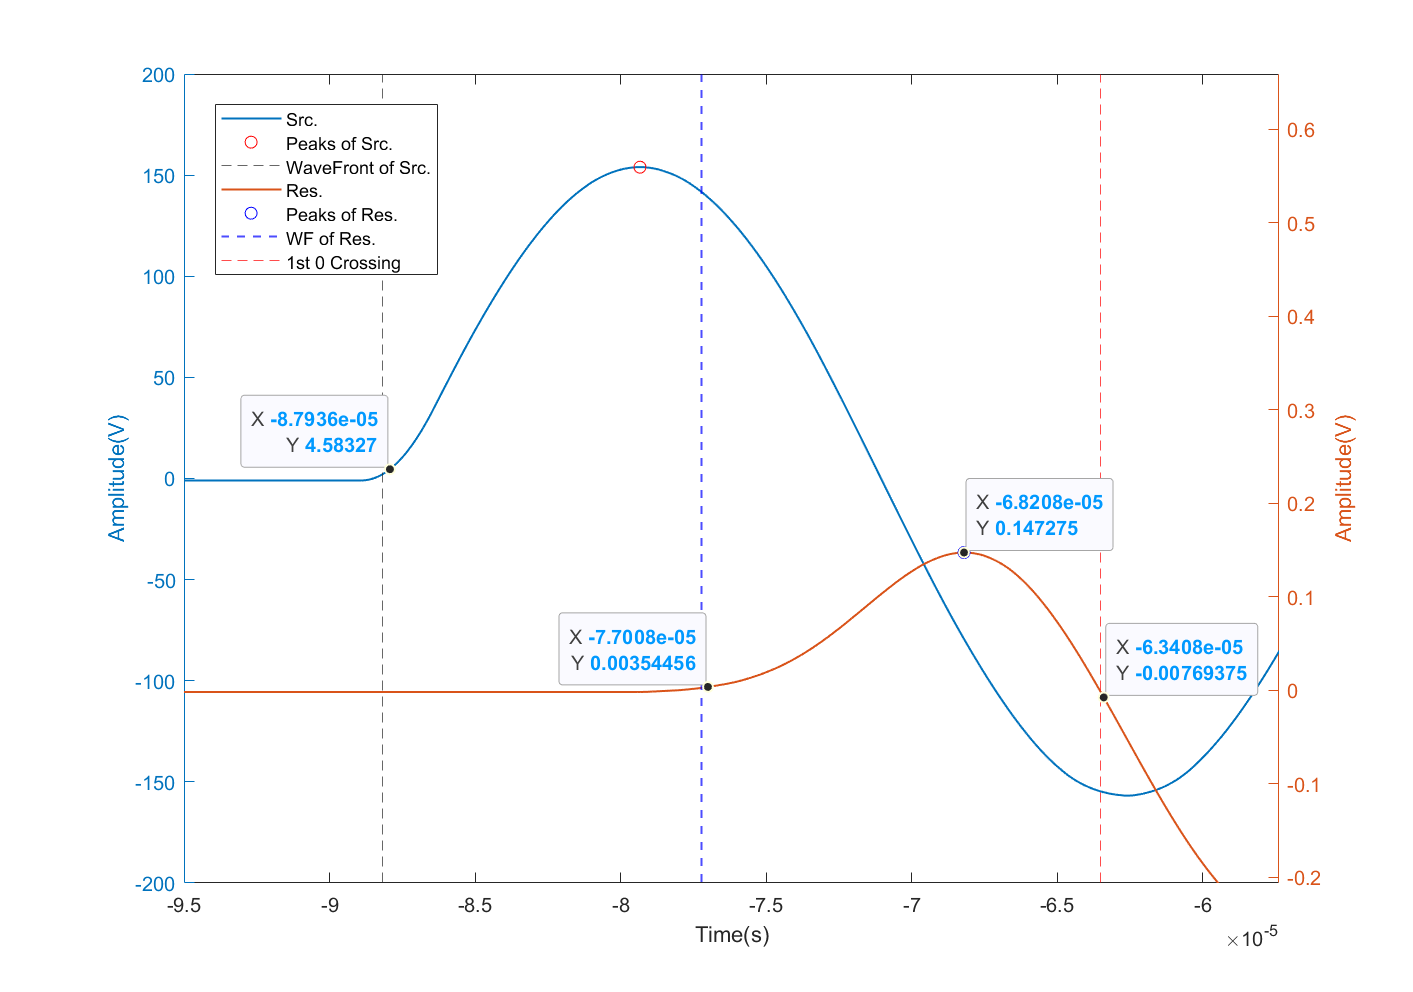
\includegraphics[height=8cm]{2_reference_point.png}
  \bicaption{同步采集源信号与响应信号,以及波前到达时刻,波峰到达时刻与首次过零时刻}{Synchronized acquisition of source and response signals, as well as wavefront arrival, peak arrival and first zero crossing moments}
  \label{fig:reference_point}
\end{figure}

我们按照上述三种到达时间的识别方法,测定了在不同厚度下的声速。特别地,我们额外使用时差法拟合得到了声速 $V_{L}$,并将其与飞行时间法测定的声速 $V_{\text{T.O.F.}}$ 进行比较。结果如图~\ref{fig:sound_velocity_measurement} 所示。实验中所使用的颗粒为 $d=2\unit{\milli\meter}$ 的钢珠,施加的单轴应力为 $P=9\unit{\kilo\Pa}$,试探信号设定为 $5$ 循环 $30\unit{\kilo\Hz}$ 正弦波列。每一个厚度都重新制备 $7$ 个不同的随机密堆积以进行系综平均,从而尽可能消除颗粒介质本身随机性的误差。

\begin{figure}[!hbtp]
  \centering
  \bisubcaptionbox{以三种参考点通过时差法求得的声速 $V_{L}$}%
                  {Sound velocity $V_{L}$ measured by time difference method with three reference points}%
                  [6cm]{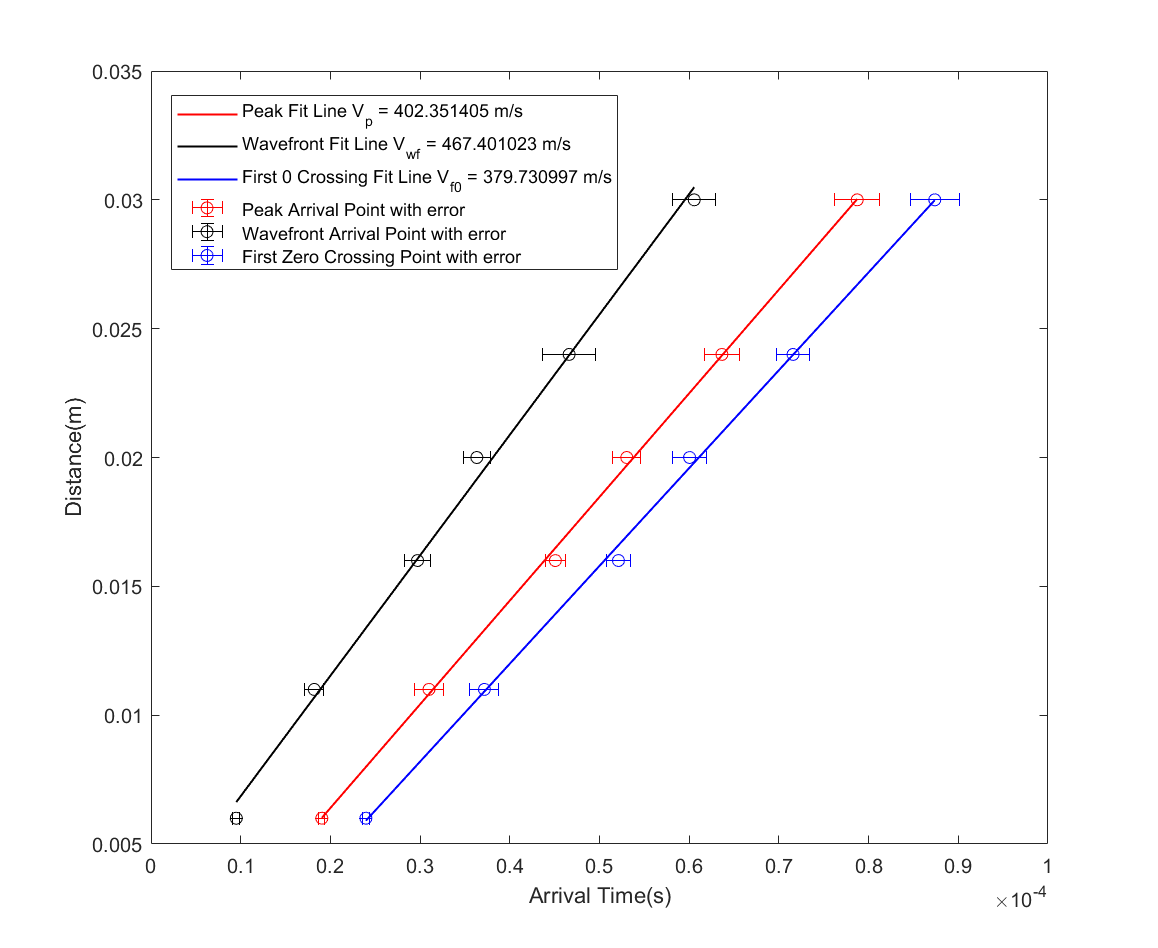
\includegraphics[height=6cm]{2_fitted_velocity.png}}
  \hspace{1cm}
  \bisubcaptionbox{以三种参考点通过飞行时间法求得的声速 $V_{\text{T.O.F.}}$}%
                  {Sound velocity $V_{\text{T.O.F.}}$ measured by Time of Flight method with three reference points}%
                  [6cm]{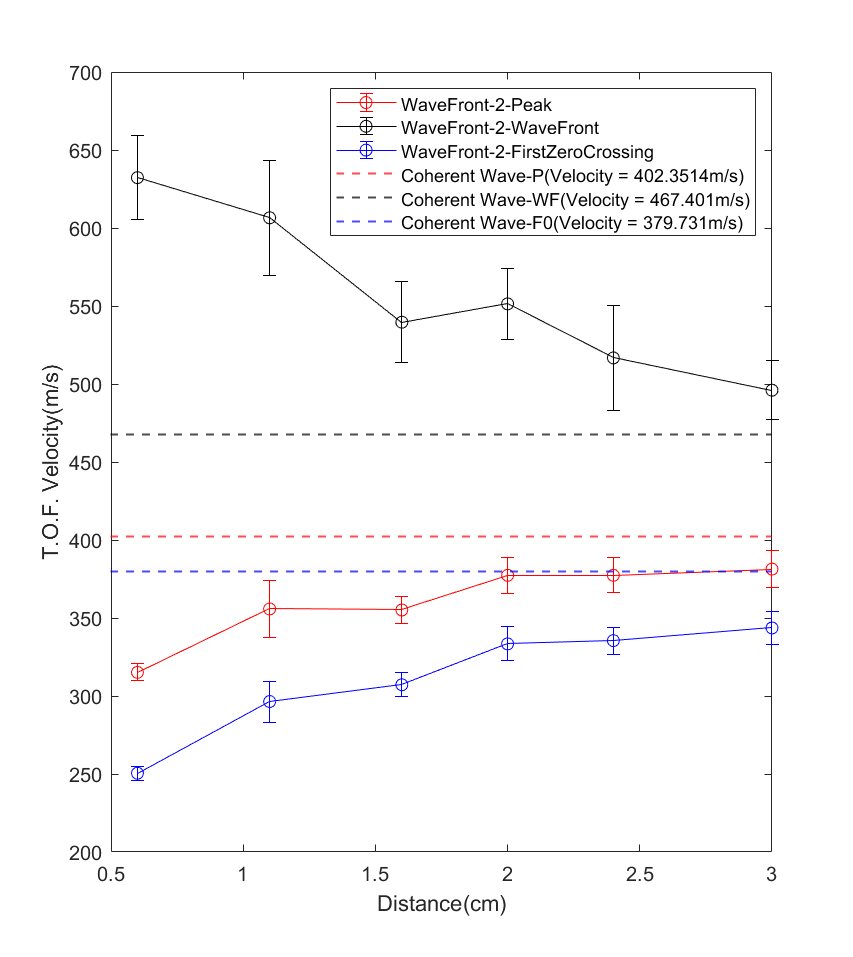
\includegraphics[height=6cm]{2_tof_velocity_and_fitted_velocity.png}}
  \bicaption{$5$ 循环 $30$ 千赫兹正弦波列作为试探信号,颗粒介质为直径 $2$ 毫米钢珠的随机密堆积,单轴应力 $9$ 千帕下的声速测量}
            {Velocity of sound measurements at $9\unit{\kilo\Pa}$ uniaxial stress with $5$-cycle of a $30\unit{\kilo\Hz}$ sine wave train as a test signal and a randomized stack of $2\unit{\milli\meter}$ diameter steel beads as the granular medium}
  \label{fig:sound_velocity_measurement}
\end{figure}

由此可见,各参考点的飞行时间法定义下的声速随着传播距离 $L$ 的增大向其时差法定义下的声速 $V_{L}$ 逼近,其中以波峰到达时间 $t_{1}$ 定义的声速在距离上的变化最为稳定,因此在传播距离足够大时,我们可以使用飞行时间法替代时差法进行工程上的声速测量,而其中以波峰到达时间定义的又是最好的。

需要额外说明的是,不同的参考点对于时差法都可以适用,但是其大小顺序和参考点的时间顺序明显相关,我们将其概括为相干首波在颗粒介质中随着传播距离增大而出现的展宽,即颗粒介质中出现了色散现象;我们将在后文通过归一化宽度更详细地探讨这一点。

% \begin{figure}[!hbtp]
%   \centering
%   \subcaptionbox{健康/损伤信号}%
%                 [7cm]{\includegraphics[height=6cm]{figures/signal_1.png}}
%   \hspace{1cm}
%   \subcaptionbox{散射信号}%
%                 [7cm]{\includegraphics[height=6cm]{figures/signal_2.png}}
%   \caption{响应信号处理}
%   \label{fig:bisubcaptionbox}
% \end{figure}

\subsection{频散能量图法}

\subsubsection{测量相速度的原理推导}

如果我们将颗粒介质中的声学传播简单考虑为单频平面波,即

\begin{equation}
  s(x,t) = A_{0}{\ee}^{-\alpha x}{\ee}^{\ii(\omega x/V_{\varphi}-\omega t)},
  \label{eq:spherical_wave}
\end{equation}

考虑在距离声源 $x_{1}$ 与 $x_{2}$ 处的两个接收探头,分别接收到声波信号 $S_{1}(t)$ 与 $S_{2}(t)$。则能求解相速度为

\begin{equation}
  V_{\varphi} = \frac{x_{2}-x_{1}}{\Delta \varphi}\omega.
\end{equation}

我们很容易想到通过 FFT 算法求解两次信号的相位频谱 $\varphi_{i}(\omega)$, 但是显然

\begin{equation}
  \Delta \varphi = \varphi_{2}(\omega) - \varphi_{1}(\omega) + 2N(\omega)\uppi
\end{equation}

对于 $N(\omega)$ 的确定则较为困难,因此地震学提出使用频散能量图观察相速度可能的分布情况。引入互关联函数 $C_{i,j}(\tau)$:

\begin{equation}
  C_{i,j}(\tau) = \int_{-\infty}^{+\infty}S_{i}(t)S_{j}(t+\tau)\mathrm{d}t.
\end{equation}

其中 $\tau$ 是描述信号延迟/传播时间的参数。该函数是一个时域函数,对其进行非幺正角频率傅里叶变换:

\begin{align}
  \mathcal{F}[C_{1,2}(\tau)] &= \int_{-\infty}^{+\infty}{\ee}^{-\ii\omega\tau}\int_{-\infty}^{+\infty}S_{1}(t)S_{2}(t+\tau)\mathrm{d}t\mathrm{d}\tau \nonumber \\
  &= \int_{-\infty}^{+\infty}S_{1}(t)\int_{-\infty}^{+\infty}{\ee}^{-\ii\omega\tau}S_{2}(t+\tau)\mathrm{d}\tau\mathrm{d}t \nonumber \\
  &= \int_{-\infty}^{+\infty}S_{1}(t)S_{2}(\omega){\ee}^{\ii\omega t}\mathrm{d}t \nonumber \\
  &= S_{1}^{*}(\omega)S_{2}(\omega).
\end{align}

通过狄拉克函数 $\delta(\omega-\omega_{n})$ 提取角频率为 $\omega_{n}$ 信号分量的延迟时间的信息,再对其进行逆非幺正角频率傅里叶变换:

\begin{align}
  \mathcal{F}^{-1}\left\{\delta(\omega-\omega_{n})\mathcal{F}[C_{1,2}(\tau)]\right\} &= \frac{1}{2\uppi}\int_{-\infty}^{+\infty}S_{1}^{*}(\omega)S_{2}(\omega)\delta(\omega_{n}){\ee}^{\ii\omega\tau}\mathrm{d}\omega \nonumber \\
  &= \frac{1}{2\uppi}S_{1}^{*}(\omega_{n})S_{2}(\omega_{n}){\ee}^{\ii\omega_{n}\tau}.
\end{align}

具体绘制时我们只需通过 $S_{1}^{*}(\omega_{n})S_{2}(\omega_{n}){\ee}^{\ii\omega_{n}\tau}/2\uppi$ 最大值归一化后的实部即可。其物理含义是,延迟时间为 $\tau$ 时,即该频率分量 $\omega_{n}$ 对应的相速度为 $V_{\varphi} = \Delta x/\tau$ 的可能性大小,所以得到的将是 $[-1,1]$ 之间的数值。通过设置离散频率分布 $\{\omega_{n}\}$, 即可查看在颗粒介质中可能的相速度分布。需要说明的是,频散能量图没有从根本上解决 $N(\omega)$ 的确定问题,但是为辅助飞行时间法测定声速提供了更直观的参考工具。

\subsubsection{颗粒介质中相速度分布}


\begin{figure}[!hbtp]
  \centering
  \bisubcaptionbox{在 $x_1=1.1\unit{cm}$ 与 $x_{2}=2.0\unit{cm}$ 处采集的响应信号}{Reponse signal captured at $x_1=1.1\unit{cm}$ and $x_{2}=2.0\unit{cm}$}%
                [7cm]{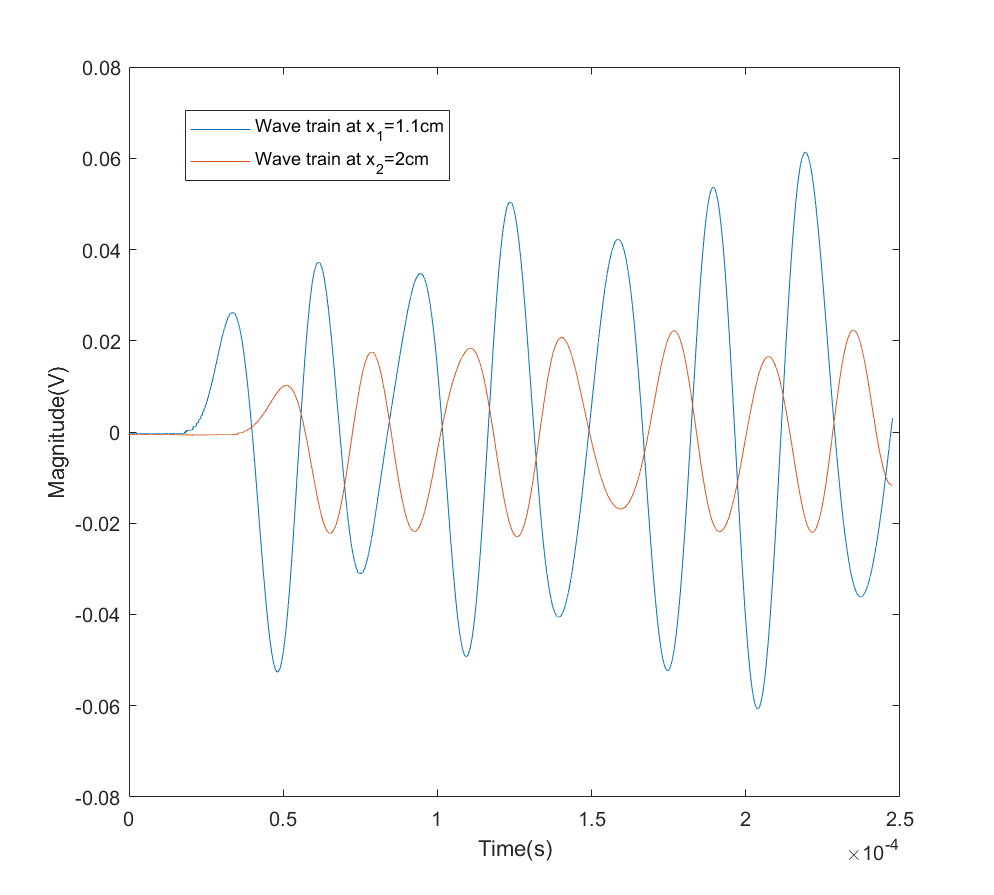
\includegraphics[height=6cm]{figures/2_wave_train.png}}
  \hspace{1cm}
  \bisubcaptionbox{$0-60\unit{kHz}$ 的相速度频域分布热图}{Phase velocity frequency distribution heat map at $0-60\unit{kHz}$}%
                [7cm]{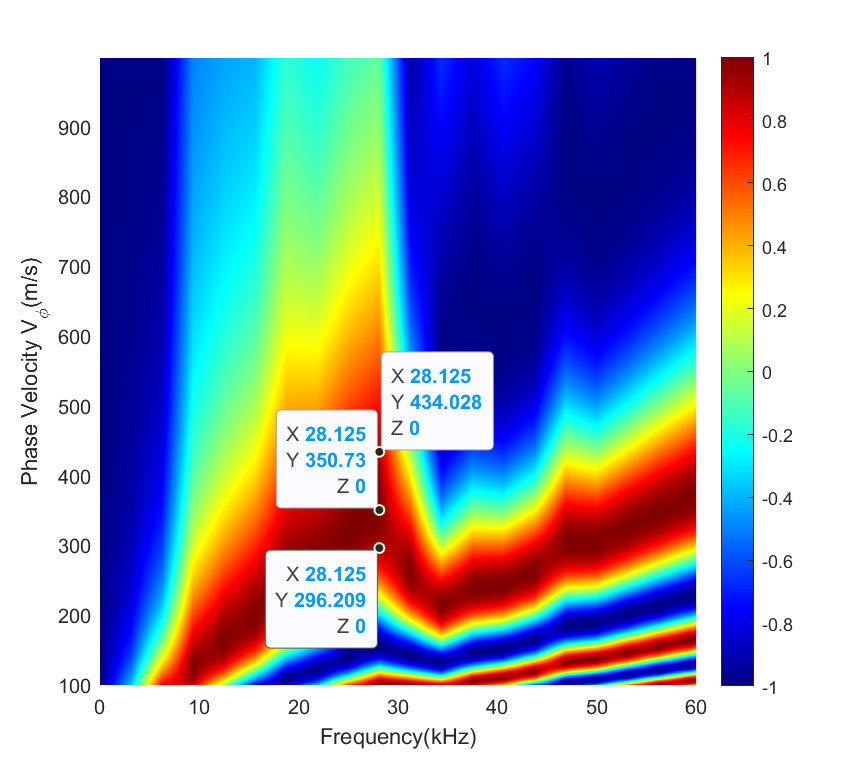
\includegraphics[height=6cm]{figures/2_cwt_v_phi.png}}
  \bicaption{根据异地响应信号计算频散能量图}{Dispersion energy map calculated from separated response signals}
  \label{fig:dispersion_energy}
\end{figure}

图 \ref{fig:dispersion_energy} 展示了在单轴应力容器中,根据不同采集距离下的两道压缩波信号绘制的频散能量图。可以看到两道信号在发射信号的中心频率 $f_{c} = 30\text{ kHz}$ 处的相速度约为 $V_{\varphi} = 350\pm 10\unit{m/s}$。

\section{声速与单轴应力的指数关系}

\subsection{等效介质理论(EMT)}

假定声波波长 $\lambda\gg$ 颗粒直径 $d$,颗粒体系由相同颗粒组成,满足紧束缚条件,颗粒介质应变可采用仿射近似,则纵波声速 $V_{L}$ 与横波声速 $V_{T}$ 分别为

\begin{align}
  V_{L} &= \sqrt{\frac{(K+\frac{4}{3}G)}{\rho^{*}}},\\
  V_{T} &= \sqrt{\frac{G}{\rho^{*}}},
\end{align}

其中 $K$ 与 $G$ 分别是颗粒介质的体弹性模量与剪切弹性模量,$\rho^{*}=\rho\phi$ 是颗粒固体的密度,$\rho$ 是颗粒材料的密度,$\phi$ 是颗粒的体积分数。在 EMT 中 模量如下给出:

\begin{align}
  K &= \frac{C_{n}}{12\uppi}\left(\phi Z\right)^{\frac{2}{3}}\left(\frac{6\uppi P}{C_{n}}\right)^{\frac{1}{3}},\\
  G &= \frac{C_{n} + \frac{3}{2}C_{t}}{20\uppi}\left(\phi Z\right)^{\frac{2}{3}}\left(\frac{6\uppi P}{C_{n}}\right)^{\frac{1}{3}},
\end{align}

其中 $Z$ 是颗粒的平均接触数,$C_{n}$、$C_{t}$ 分别是描述颗粒在法向和切向与力相关的系数。Hertz 接触和 Mindlin 接触分别使用了这两个系数,即两个颗粒通过接触完成的相互作用为

\begin{align}
  f_{n} &= \frac{2}{3}C_{n}R^{\frac{1}{2}}w^{\frac{3}{2}},\\
  f_{t} &= C_{t}(Rw)^{\frac{1}{2}}\Delta s,
\end{align}

其中 $w$ 是半径分别为 $R_{1}$、$R_{2}$ 的两个颗粒之间的重叠量,$R = \frac{2R_{1}R_{2}}{R_{1} + R_{2}}$ 为颗粒的等效半径。引入颗粒材料(下标 $g$)的剪切模量 $G_{g}$ 与泊松比 $\nu_{g}$,完成对力系数的表述:

\begin{align}
  C_{n} &= \frac{4G_{g}}{1-\nu_{g}},\\
  C_{t} &= \frac{8G_{g}}{2-\nu_{g}}.
\end{align}

\subsection{实验验证}

同样在单轴应力容器装置中,使用直径 $d=2\unit{\milli\meter}$ 的钢珠制备随机密堆积,并施加单轴应力 $P=$ \numlist{0.40;3.34;6.30;8.43;9.63;11.31;14.46}\unit{\kilo\pascal}。使用飞行时间法测定各应力下的声速 $V_{\text{T.O.F.}}(P)$,并观察声速与单轴应力的指数关系是否符合 EMT 的预期。

\begin{figure}[!hbtp]
  \centering
  \bisubcaptionbox{双线性轴下的应力 $P$ 与声速 $V_{\text{T.O.F.}}$ 的关系}%
                  {Stress $P$ versus sound velocity $V_{\text{T.O.F.}}$ in bilinear axis}%
                  [6.4cm]{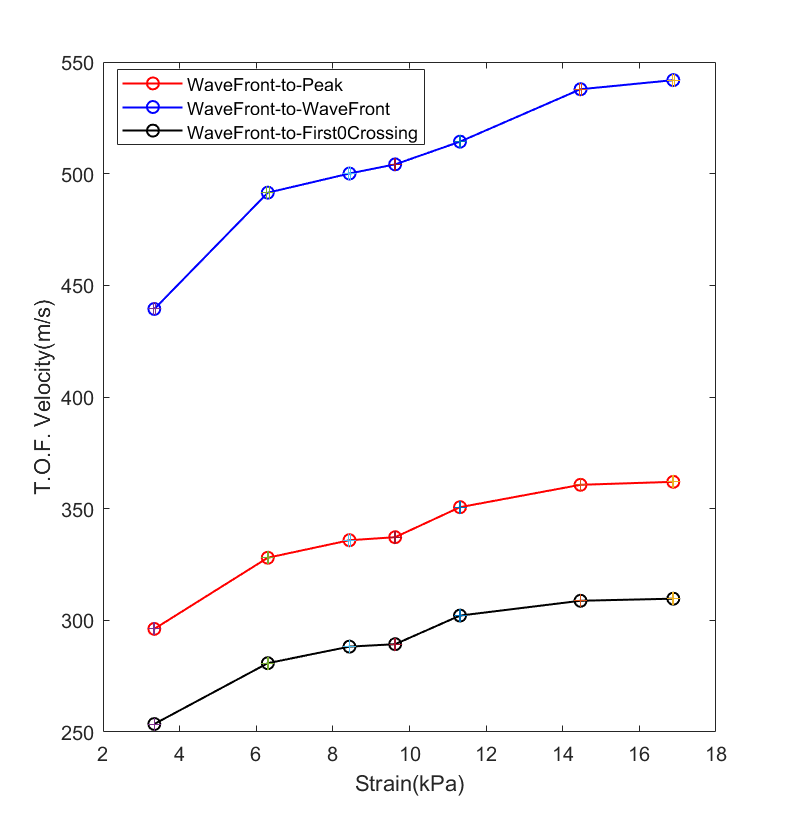
\includegraphics[height=7cm]{figures/2_strain_vs_velocity_20mm_1.png}}
  \hspace{1cm}
  \bisubcaptionbox{双对数处理后的应力 $P$ 与声速 $V_{\text{T.O.F.}}$ 的关系及其线性拟合}%
                  {Relationship between stress $P$ and sound velocity $V_{\text{T.O.F.}}$ after double logarithmic  and its linear fit}%
                  [6.4cm]{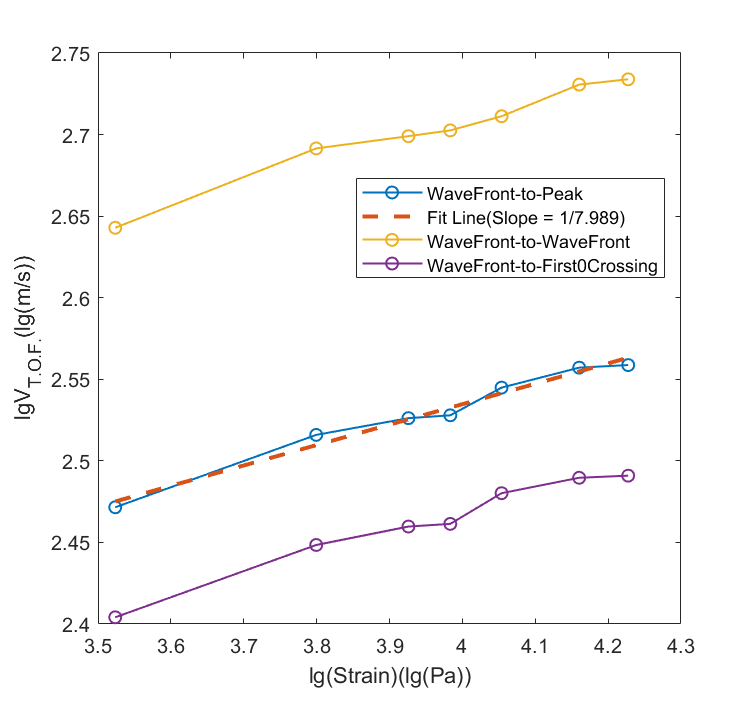
\includegraphics[height=7cm]{figures/2_strain_vs_velocity_20mm_2.png}}
  \bicaption{声速 $V_{\text{T.O.F.}}$ 与单轴应力 $P$ 的幂律关系。$P =$ \numlist{0.40;3.34;6.30;8.43;9.63;11.31;14.46}\unit{\kilo\pascal},颗粒介质为厚度 $L =19$\unit{\milli\meter} 的直径 $2$\unit{\milli\meter} 钢珠随机密堆积}
                  {Power-law relationship between the sound velocity $V_{\text{T.O.F.}}$ and the uniaxial stress $P$. $P =$ \numlist[
                    list-final-separator = { and }
                  ]{0.40;3.34;6.30;8.43;9.63;11.31;14.46}\unit{\kilo\pascal}, where the granular medium is a random close packing with steel beads of diameter $2\unit{\milli\meter}$ and thickness $L = 19$\unit{\milli\meter}}
  \label{fig:normalized_width_versus_L}
\end{figure}


%%% 可能是因为容器几何因素导致的 Yassen Effect,导致应力并不充分地施加到颗粒介质上。

\section{超声脉冲在颗粒介质中的展宽}

颗粒介质通过异质性的力链网络传递应力,因此声波在颗粒介质中传播时会因为其非线性出现剧烈的畸变现象,其中脉冲超声波的展宽是较为明显的现象之一。本节讨论了颗粒介质厚度 $L$ 以及单轴应力 $P$ 对于脉冲波展宽的影响。

\subsection{归一化宽度的定义}

在信号处理中,常见的对于峰宽度的定义通常是半高宽;事实上,我们在处理响应信号的到达时间时,使用的寻峰算法中的参数也的确包含了半高宽阈值用于排除噪音的干扰。但是这里我们引入的归一化宽度参数 $W$ 同时考虑了峰值与波前在时域中位置:

\begin{equation}
  W \equiv \frac{t_{1}-t_{0}}{t_{1}},
\end{equation}

其中 $t_{0}$ 与 $t_{1}$ 分别为波前与峰值的到达时间。我们在测定最佳信号参考点的时候应当意识到,脉冲的展宽实际上已经在一定程度上反映了“在颗粒介质中存在着较明显的色散关系”;而峰值到达时间定义的飞行时间速度,即在试探信号中心频率附近,在距离上更具有稳定性。因此,通过与中心频率(这里指所发射的试探信号的频率 $f_{c}$)关联的 $t_{1}$ 来对信号进行缩放操作是合理的。后文通过数据处理后得到的图~\ref{fig:reference_point} 以及对应讨论中进一步证明这一点。

\subsection{归一化宽度与颗粒介质厚度的关系}

\subsubsection{理论推导}

我们先从最简单的一维弹簧链开始推导。凝聚态物理中,我们已经知道一维晶格的色散关系为

\begin{equation}
  \omega=\sqrt{\frac{4C}{M}}\left|\sin\left(\frac{ka}{2}\right)\right|,
\end{equation}

其中 $C$ 为弹性系数,$M$ 为弹簧所连接质点的质量,$a$ 为质点间距/晶格常数。我们将其写为反函数形式:

\begin{equation}
  k(\omega) = \frac{2}{a}\arcsin{\left(\sqrt{\frac{M}{4C}}\omega\right)}.\label{eq:1D_dispersion_relation}
\end{equation}

在这里,我们对式~\eqref{eq:1D_dispersion_relation} 应用长波极限 $ka\ll 1$, 从而求得波速度:

\begin{equation}
  V = \lim_{ka\ll 1}\frac{\omega}{k} = \sqrt{\frac{C}{M}}a.
\end{equation}

使用 $V$ 替换式~\eqref{eq:1D_dispersion_relation} 中的 $C$,$M$ 项,且假定长波极限下的声速 $V$ 充分大,使得我们足以通过麦克劳林级数将其展开至前两项:

\begin{equation}
  k = \frac{2}{a}\left[\frac{a\omega}{2V} + \frac{1}{6}\left(\frac{a\omega}{2V}\right)^{3} + o\left(\frac{1}{V^3}\right)\right]\approx\frac{\omega}{V} + \frac{2\omega^{3}a^{2}}{3V^{3}},
\end{equation}

将其代入至波数项中,我们将看到

\begin{equation}
  \text{exp}\left[{\ii \left(\frac{\omega}{V} + \frac{2a^{2}\omega^{3}}{3V^{3}}\right)x}\right] = \text{exp}[{\ii\omega t_{1}}]\text{exp}\left[{\ii\left(\frac{\omega}{\omega_{1}}\right)^{3}}\right],\quad t_{1} = \frac{x}{V},\quad \omega_{1} = \sqrt[3]{\frac{3V^{3}}{2a^{2}x}}.\label{eq:rescale_method}
\end{equation}

而我们已经知道,在傅里叶变换中,存在关系

\begin{align}
  \mathcal{F}[f(t+t_{1})] = \mathcal{F}[f(t)]{\ee}^{\ii\omega t_{1}},\label{eq:translation_property}\\
  \mathcal{F}[f(\omega_{1}t)] = \frac{1}{|\omega_{1}|}\hat{f}\left(\frac{\omega}{\omega_{1}}\right),\label{eq:scale_property}\\
  \mathcal{F}[\text{Ai}(t)] = \text{exp}\left[\ii\cdot \frac{1}{3}\omega^3\right].
\end{align}

将波数项代入至 $a(x,-t)$ 中,并对其进行傅里叶变换:

\begin{equation}
  \mathcal{F}[a(x,-t)] = \int_{-\infty}^{+\infty}A_{0}{\ee}^{\ii\omega t_{1}}{\ee}^{\ii(\omega/\omega_{1})^{3}}e^{\ii\omega t}e^{-\ii\omega t}\mathrm{d}t = A_{0}{\ee}^{\ii\omega t_{1}}{\ee}^{\ii(\omega/\omega_{1})^{3}}.
\end{equation}

所以,根据傅里叶变换的平移性质~\eqref{eq:translation_property}与尺度性质~\eqref{eq:scale_property},我们得到源信号形式可近似为通过 $\omega_{1}$ 控制宽度的 Airy 函数:

\begin{equation}
  s(x,t) = \omega_{1}\text{Ai}\left[\omega_{1}(t_{1}-t)\right].
\end{equation}

因此,在一维弹簧链中,脉冲波传播到距离 $L$ 处的归一化宽度为

\begin{equation}
  W \approx \frac{\pi}{2\omega_{1}}\frac{1}{t_{1}}\propto L^{-2/3}.
\end{equation}

考虑一维球链时,使用 $a=2R$ 替换即可得到对应的公式\cite{PhysRevE.91.022205}。接下来我们进一步考虑颗粒介质中衰减项 $\alpha$ 的影响。引入弹性模量的涨落 $\nu_{K} = \Delta K^{-1}/\bar{K}^{-1}$ 与对应的关联长度 $L_{c}$,我们可以得到一维随机层理论对于衰减项的描述:

\begin{equation}
  \alpha(\omega) = k^{\prime\prime}(\omega) = [\sigma_{K}^{2}L_{c}^{n-1}]\left(\frac{\omega}{V}\right)^{n}.
\end{equation}

其中满足

\begin{align}
  V &= \bar{V} = \sqrt{\frac{\bar{K}}{\bar{\rho}}}\\
  \gamma &= \int_{0}^{+\infty}\langle\nu_{K}(0)\nu_{K}(x)\rangle\mathrm{d}x = \sigma_{K}^{2}L_{c}
\end{align}

通过引入虚波矢 $k^{\prime\prime}$ 写出频域内的信号分布,并仿照上面一维弹簧链中的式~\eqref{eq:rescale_method} 进行缩放操作:

\begin{equation}
  \widetilde{a}(\omega) = {\ee}^{ik^{\prime}x}e^{-k^{\prime\prime}x} = e^{i\omega t_{1}}e^{-\left(\frac{\omega}{\omega_{1}}\right)^{n}},\quad t_{1} = \frac{x}{V},\quad \omega_{1} = \sqrt[n]{\frac{V^{n}}{\sigma_{K}^{2}L_{c}^{n-1}x}}.
\end{equation}

因此得到归一化宽度:

\begin{equation}
W\sim \frac{1}{\omega_{1}t_{1}} = (\sigma_{K})^{\frac{2}{n}}\left(\frac{n-1}{n}\right)^{\frac{n-1}{n}}
\end{equation}

在一维随机分层介质中有 $n=2$, 因此在 $x = L$ 处归一化宽度为

\begin{equation}
  W\propto L^{-\frac{1}{2}}.
\end{equation}

\subsubsection{实验验证}

我们控制试探信号为 $5$ 循环 $30\unit{\kilo\Hz}$ 连续正弦波列作为试探信号,使用颗粒为直径 $2\unit{\milli\meter}$ 的钢珠生成随机密堆积,施加的单轴应力为 $9\unit{\kilo\Pa}$;分别测定了颗粒介质厚度为 $\numlist{6;11;16;20;24;30}\unit{\milli\metre}$ 时的响应信号,并且每一厚度都各自单独重新制备 7 次随机密堆积以尽可能消除实验误差,并且数据进行系综平均,标准差作为误差棒。图~\ref{fig:reference_point} 展示了其中一组响应信号通过相干波峰 $A_{1}$ 归一化,且时间轴以波峰到达时间 $t_{1}$ 进行缩放后的图像:

\begin{figure}[!htp]
  \centering
  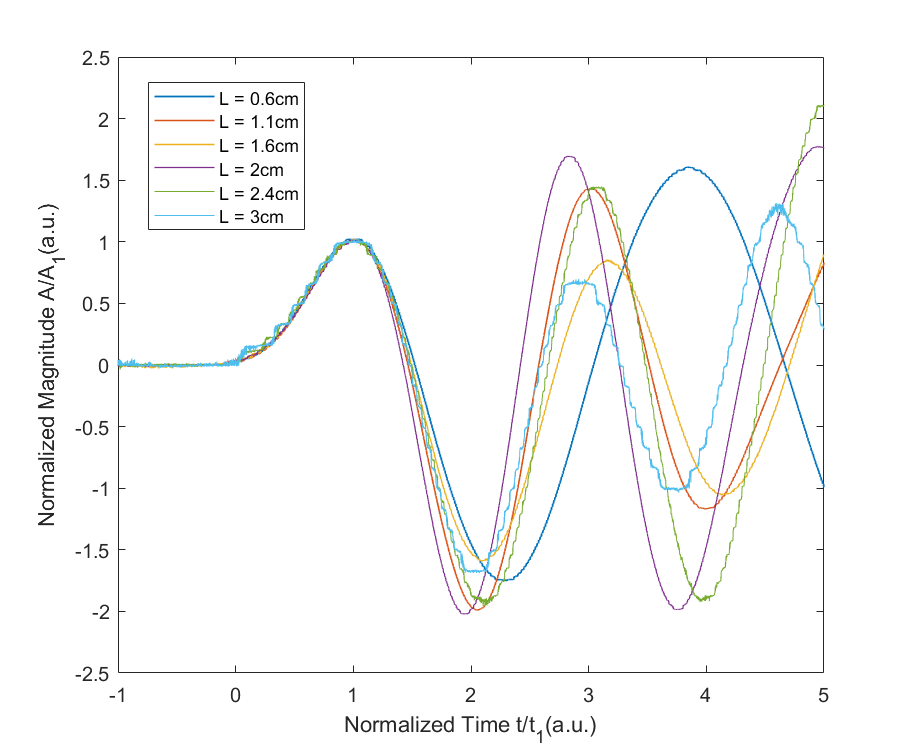
\includegraphics[height=6cm]{2_Rescaled_Magnitude_differing_in_Distance.png}
  \bicaption{通过相干波峰 $A_{1}$ 归一化,且时间轴以波峰到达时间 $t_{1}$ 进行缩放后的不同颗粒样品厚度下测得的响应信号}{Response signal captured at different granular sample thicknesses, normalized with coherent wave peak $A_{1}$ and time axis rescaled with peak arrival time $t_{1}$}
  \label{fig:reference_point}
\end{figure}

可以发现,虽然采集信号时的颗粒介质厚度各异,但是通过幅值归一化与时间轴的缩放,仍能够观察到“响应信号可以提取出相干首波”的本质特征。当 $t/t_{1} > 1$,响应信号的宽度开始出现显著变化;而在前面的信号参考点选取的实验中,我们已经知道,$t_{1}$ 是一个性质较为良好的参考点,因此我们可以通过借助 $t_{1}$ 定义的归一化宽度 $W$ 来探究其与颗粒介质厚度,即信号传播距离 $L$ 之间的关系。

图~\ref{fig:normalized_width_versus_L} 展示了上述实验中测得的归一化宽度 $W$ 与颗粒介质厚度 $L$ 之间的关系,其中为了观察幂律关系使用了双对数处理并对其数据点进行了线性拟合。不难看出,我们得出的结果约为 $W\propto L^{-0.448}$,与理论推导的 $W\propto L^{-1/2}$ 已经相当接近。

需要说明的是,这种偏差存在两种来源:

\begin{enumerate}
  \item 波前到达时间的选取并不是绝对的。既然我们是通过 $S(t_{0}) = A_{1}\cdot k$($k\in(0,0.1]$)确定的 $t_{0}$,那么 $k$ 的具体数值会影响到 $t_{0}$ 的选取,从而影响到归一化宽度 $W$ 的测定;而在传播距离较大时,响应信号的信噪比会因为信号衰减而急剧降低,此时对全体传播距离上的响应信号划定一条通用可行的 $k$ 实际上是存在困难的,因此其具体数值需要通过经验来调整;
  \item 理论推导中的 $n=2$ 是一维随机分层介质的情况。虽然我们已经将色散关系和衰减同时纳入考虑,并且实验模式中超声波的传播偏向于柱坐标中单个 $z$ 轴方向上,但是着一切仍不能改变“实际的颗粒介质仍然是三维体系”的事实,因此出现 $-0.448\sim-1/2$ 的偏差是在理解范围内的。
\end{enumerate}

\begin{figure}[!hbtp]
  \centering
  \bisubcaptionbox{相干首波峰宽度 $t_{1} - t_{0}$}%
                  {Coherent wave peak width $t_{1} - t_{0}$}%
                  [6.4cm]{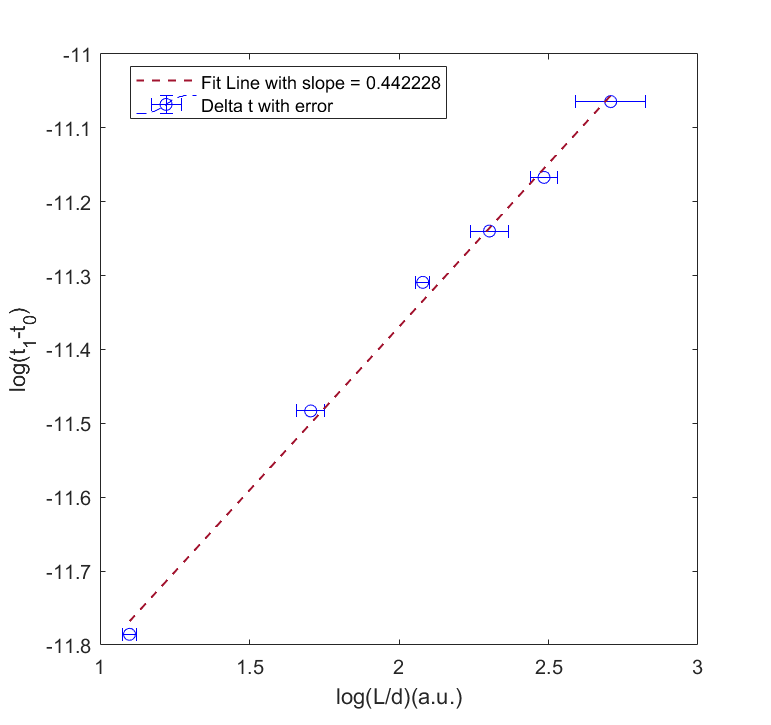
\includegraphics[height=7cm]{figures/2_t1-t0_L.png}}
  \hspace{1cm}
  \bisubcaptionbox{相干首波归一化宽度 $W$}%
                  {Coherent first wave normalized width $W$}%
                  [6.4cm]{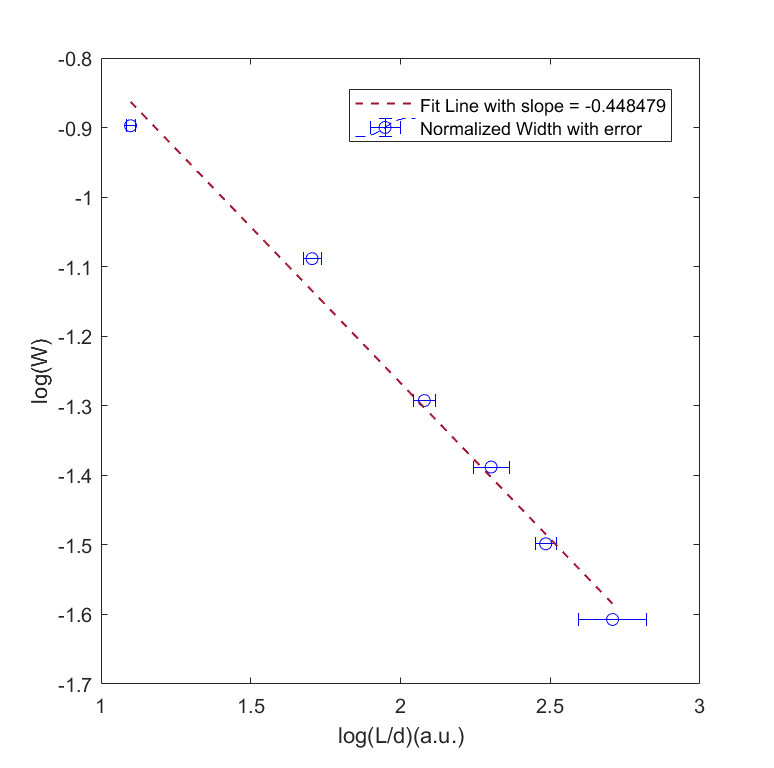
\includegraphics[height=7cm]{figures/2_W_L.png}}
  \bicaption{颗粒介质厚度为 \numlist{6;11;16;20;24;30} \unit{\milli\metre} 时的响应信号首峰宽度 $t_{1} - t_{0}$ 与归一化宽度 $W$}
                  {First peak width $t_{1} - t_{0}$ and normalized width $W$ of response signal at granular medium thickness of \numlist[
                    list-final-separator = { and }
                  ]{6;11;16;20;24;30} \unit{\milli\metre}}
  \label{fig:normalized_width_versus_L}
\end{figure}

\subsection{归一化宽度与单轴应力的关系}

类似于上述实验中考虑的颗粒介质厚度,即脉冲传播距离对脉冲归一化宽度的影响,我们也对在不同单轴应力 $P$ 下的归一化宽度 $W(P)$ 进行了计算与绘图,数据来自于单轴应力与声速关系的实验。但遗憾的是,如图~\ref{fig:normalized_width_versus_P} 所示,我们没有观察到明显的规律。

\begin{figure}[!hbtp]
  \centering
  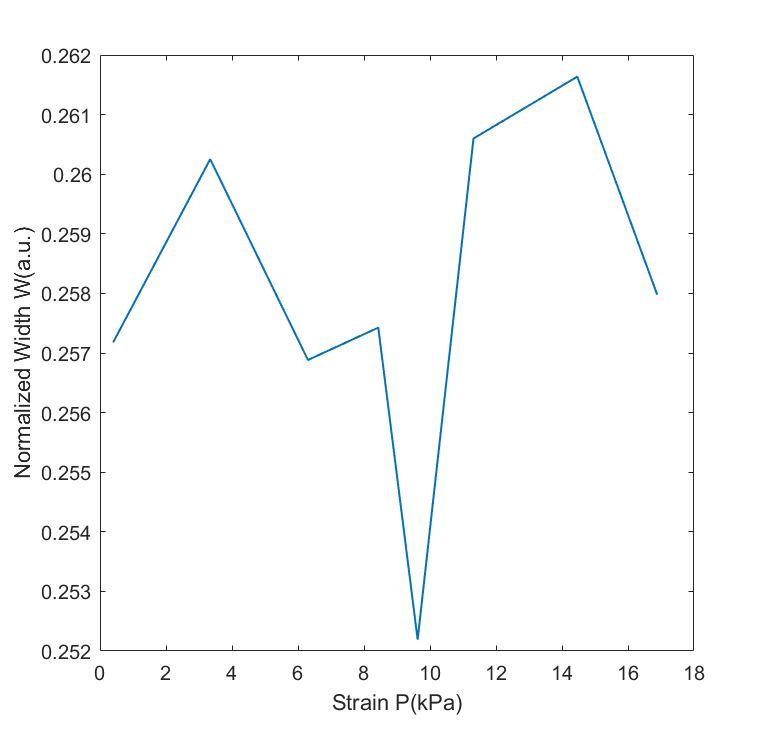
\includegraphics[height=7cm]{figures/2_W_norm&Strain.png}
  \bicaption{单轴应力 $P$ 与归一化宽度 $W$ 的关系}{Relationship between uniaxial stress $P$ and normalized width $W$}
  \label{fig:normalized_width_versus_P}
\end{figure}

目前对于该现象的解释是,颗粒介质中本身存在着如 Jassen Effect 等现象,即在诸如圆筒形容器中颗粒介质所受重力并非完全沿轴向传递,而是会有一部分力被颗粒介质中的结构分配到径向。这与通常的液压规律完全不同,因此早期人类的粮仓会因为设计不合理而被过量的径向应力破坏、坍塌\cite{sperlExperimentsCornPressure2006}。在我们的实验中,由于容器的几何因素,可能类似的效应使得颗粒介质对于脉冲信号的响应规律性受到影响,导致所观察到的 $W(P)$ 与 $P$ 之间的关系并不明显。
% !TEX root = ../main.tex

\chapter{散射尾波}

\section{超声波在颗粒介质中的扩散近似}

\subsection{理论推导}

Weaver R. L. 推导出了超声波脉冲在多晶体中的扩散行为方程\cite{diffusivity}:

\begin{equation}
  \frac{\partial I}{\partial t} - D\nabla^{2}I + \frac{I}{\tau_{\alpha}} = \delta(z)\delta(t)
\end{equation}

其中 $D$ 是扩散系数,$\tau_{\alpha}$ 是描述强度在时域上衰减的特征时间,$z$ 是圆柱坐标系中的径向坐标。因为是脉冲超声波(脉冲宽度充分小,中心频率充分大),即视为时域和空间上的 Dirac 函数 $\delta{z}\delta(t)$。

因为在实际的实验中,我们使用的颗粒容器是圆筒形,所以在求解强度方程时可以采用圆柱对称处理;又因为亚克力板容器壁厚达 10 \unit{\milli\meter} 而假定容器边界的声阻抗足够大,在这种情形下声信号在容器壁全反射。则进入底部探头的透射通量\cite{PhysRevLett.93.154303}为

\begin{equation}
  J(t) = \frac{\nu U_{0}}{2L}{\ee}^{-\frac{t}{\tau_{\alpha}}}\sum_{n=0}^{\infty}\frac{(-1)^{n}}{\delta_{n}}\cos{\left(\frac{n\uppi l^{*}}{L}\right)}{\ee}^{-\frac{D(n\uppi)^{2}t}{L^{2}}},\quad \delta_{n} = \begin{cases}
    2, & n = 0, \\
    1, & \text{otherwise}.
  \end{cases}
\end{equation}

其中 $U_{0}$ 是声源能量, $D = \frac{1}{3}\nu_{e}l^{*}$ 为扩散系数, $\nu_{e}$ 为能量传输速度, $l^{*}$ 为平均自由程, $\tau_{\alpha}$ 正式名为非弹性吸收时间。在实验中,我们用飞行时间法测定的声速 $V_{\text{T.O.F.}}$ 来替代 $\nu_{e}$。


\subsection{实验验证}



\section{超声波在颗粒介质中的非线性}

%\subsection{线性响应理论}
% 老师声称这个可以用来水字数,但是是这样吗?

\subsection{非线性波方程与各级谐波}

在连续介质力学中,我们已经学习过描述声波传播的 Burgers 方程:

\begin{align}
  \frac{\partial p}{\partial x} - \frac{\delta}{2c_{0}^{3}}\frac{\partial^{2}p}{\partial t^{2}} = \frac{\beta p}{\rho_{0}c_{0}^{3}}\frac{\partial p}{\partial t},\label{eq:burgers_equation_1}\\
  \delta = \frac{1}{\rho_{0}}\left[\frac{4}{3}\mu + \mu_{B} + \kappa\left(\frac{1}{c_{v}} - \frac{1}{c_{p}}\right)\right].
\end{align}

其中 $\mu$ 是介质的剪切黏度,$\mu_{B}$ 是介质的容变黏度,这两者共同构成了介质的黏性吸收;$\kappa$ 是介质的热导率,$c_{v}$ 是介质的定容热容,$c_{p}$ 是介质的定压热容,这两者构成了介质的热传导吸收。两者的线性叠加构成了 Stokes-Kirchhoff 衰减公式,用于描述声波在介质中传播时的经典吸收现象。$\beta$ 是介质的非线性系数,$\rho_{0}$ 和 $c_{0}$ 分别是介质在平衡态下的密度和声速。

Mendousse 首个推导出专用于平面波声传播的偏微分方程。他设定具有黏度的理想气体,根据 Navior-Stockes 方程写出一维流动形式的 Lagrangian 量:

\begin{equation}
  \rho_{0}\frac{\partial^{2}\xi}{\partial t^{2}} - \frac{4}{3}\mu\frac{\partial }{\partial a}\left[\left(1 + \frac{\partial\xi}{\partial a}\right)\frac{\partial^{2}\xi}{\partial a\partial t}\right] + \frac{\partial P}{\partial a} = 0.\label{eq:mendousse_equation}
\end{equation}

其中,$\xi$ 是参考于物质位置 $a$ 的流体粒子位移量,即存在坐标关系为

\begin{equation}
  x = a + \xi(a,t).
\end{equation}

Mendousse 假定黏性吸收中由体变黏度 $\mu_{B}$ 和热导率 $\kappa$ 引起的吸收远小于由剪切黏度 $\mu$ 所引起的从而只保留了后者,并且在黏性项中忽略了本应存在的系数 $1+\partial\xi/\partial a$。考虑到流体中局域的质量守恒规则,我们可以得到平衡态下的密度和流变密度之间的关系:

\begin{equation}
  \rho_{0} = \left(1 + \frac{\partial\xi}{\partial a}\right)\rho,
\end{equation}

由于忽略了黏度相关的一个二阶项,总压力 $P$ 对 $\partial\xi/\partial a$ 的级数展开化为

\begin{equation}
  P = P_{0} - \rho_{0}c_{0}^{2}\left[\frac{\partial\xi}{\partial a} - \beta\left(\frac{\partial\xi}{\partial a}\right)^{2}\right],
\end{equation}

所以式~\eqref{eq:mendousse_equation} 化为下式:

\begin{equation}
  \rho_{0}\frac{\partial^{2}\xi}{\partial t^{2}} - \rho_{0}\delta\frac{\partial^{3}\xi}{\partial a^{2}\partial t} - \rho_{0}c_{0}^{2}\frac{\partial^{2}\xi}{\partial a^{2}} + 2\rho_{0}c_{0}^{2}\beta\frac{\partial\xi}{\partial a}\frac{\partial^{2}\xi}{\partial a^{2}} = 0,\label{eq:progressive_burgers_equation}
\end{equation}

对于角频率为 $\omega$ 的正弦波在诸如上述方程所控制下的传播,其产生的畸变与失真可以理解为产生高次谐波的过程。因此通过级数展开求解式~\eqref{eq:progressive_burgers_equation},依次得到基波、各级谐波的表达式:

\begin{equation}
  \begin{cases}
    u_{1\omega}(a,t) &\approx u_{\text{in}}e^{-a\alpha}\cos{(ka-\omega t)}\\
    u_{2\omega}(a,t) &\approx \frac{u_{\text{in}}^{2}}{8}\left(\frac{\beta\omega^{2}}{\alpha c_{0}^{2}}\right)e^{-2\alpha a}\cos{[2(ka-\omega t)]}\\
    u_{3\omega}(a,t) &\approx \frac{u_{\text{in}}^{3}}{48}\left(\frac{\beta\omega^{2}}{\alpha c_{0}^{2}}\right)^{2}e^{-3\alpha a}\cos{[3(ka-\omega t)]}
    \end{cases}
\end{equation}

其中 $u_{\text{in}}$ 是声源振幅,$a$ 是声波传播距离,$\alpha$ 是声波的衰减系数,$k$ 是声波的波数,$\omega$ 是声波的频率。$u_{n\omega}$ 代表 $n$ 倍频的谐波振幅($n=1$ 即为基波)。我们很容易以一个简单的公式总结各谐波振幅与源振幅的关系:

\begin{equation}
  u_{n\omega} \propto \left(u_{\text{in}}\right)^{n}.\label{eq:harmonic_linear}
\end{equation}

颗粒介质具有强耗散性,我们可以将这种信号在颗粒介质中的衰减类比于声波在具有切变黏性 $\mu$ 的流体中传播时所受的黏性吸收作用,即使用等效黏度 $\mu^{*}$ 来对颗粒介质进行宏观的统计性描述。如果式~\eqref{eq:harmonic_linear} 描述的线性关系随着声源振幅 $u_{\text{in}}$ 增大遭到破坏,即说明等效黏度已经因为泵浦作用发生变化。对于水和空气这类连续介质,在黏性力相较于弹性力很小时,存在描述衰减 $\alpha$ 与声波角频率 $\omega$ 的指数关系:

\begin{equation}
  \alpha = \alpha_{\mu} + \alpha_{h} = \frac{\omega^{2}}{2\rho_{0}c_{0}^{3}}\left[\frac{4}{3}\mu + \mu_{B} + \kappa\left(\frac{1}{c_{v}} - \frac{1}{c_{p}}\right)\right]\propto \omega^{2}
\end{equation}

其中 $\alpha_{\mu}$ 和 $\alpha_{h}$ 分别是描述黏性吸收和热传导吸收的衰减系数。在后文中我们将组织实验来验证通过接触力相联系的颗粒介质中,是否同样存在着类似的衰减系数 $\alpha^{*}$ 与信号角频率 $\omega$ 之间的指数关系。

\subsection{相似性参数}

引入交叉关联函数(cross-relation function)作为相似性参数 $\Psi_{i,j}(\tau)$, 以描述信号 $S_{i}$ 与 $S_{j}$ 的相似程度\cite{PhysRevLett.90.174302}:

\begin{equation}
  \Psi_{i,j}(\tau) \equiv \frac{\int_{-\infty}^{+\infty}S_{i}(t)S_{j}(t+\tau)\mathrm{d}t}{\sqrt{\int_{-\infty}^{+\infty}S_{i}^{2}(t)\mathrm{d}t\int_{-\infty}^{+\infty}S_{j}^{2}(t)\mathrm{d}t}}.
\end{equation}

其中 $\tau$ 描述的是采集各信号之间的延时。在真实的实验时,我们是通过某一采集频率 $f_{s}$ 对各信号进行采样的,即得到的信号形式会是一个时域上序列的离散值 $S_{i}(t_{n})$,所以实际计算时采用求和形式,即

\begin{equation}
  \Psi_{i,j}(\tau)\equiv \frac{\sum_{n=1}^{N}S_{i}(t_{n})S_{j}(\tau+t_{n})}{\sqrt{\sum_{n=1}^{N}s_{i}^{2}(t_{n})}\sqrt{\sum_{n=1}^{N}s_{j}^{2}(t_{n})}}.
\end{equation}

该函数的定义与前文通过频散能量图求解相速度分布中所用的关联函数 $C_{i,j}$ 非常相似,区别仅在于本节通过各信号平方在时域上的积分进行归一化,因此最后求得的值域范围将是 $[-1,1]$。如果相似性参数 $\Gamma_{i,j}$ 越接近 $1$,则信号 $S_{i}$ 与 $S_{j}$ 越相似,颗粒介质对于第 $i$ 次和第 $j$ 次的源试探信号的散射效果越接近,从而证明颗粒介质的力链结构变化越小。由于这种相似性参数对于颗粒介质内部的应力结构变化极为敏感,所以低振幅超声波被视为一种非侵入式的探针:在颗粒介质经历连续外部激励时,为了察觉其内部结构是否变化,可以观察时域上相邻的响应信号之间的相似性参数是否会出现骤降。

在部分研究受环形剪切的颗粒介质中的滞滑实验中,曾提到过不同类型的滞滑事件产生的声发射信号在频域上的分布相似\cite{doi:10.1073/pnas.2305134120}。只要我们意识到两时域信号相互做内积的结果量纲为能量,我们很容易通过能量守恒的观点将相似性参数的定义延拓到频域上。

首先我们证明 Parseval 定理:

\begin{equation}
  \begin{aligned}
    \int_{-\infty}^{+\infty}S_{i}(t)\bar{S}_{j}(t)\mathrm{d}t &= \int_{-\infty}^{+\infty}\left[\frac{1}{2\uppi}\int_{-\infty}^{+\infty}S_{i}(\omega){\ee}^{\ii \omega t}\mathrm{d}\omega\right]\left[\frac{1}{2\uppi}\int_{-\infty}^{+\infty}\bar{S}_{j}(\omega^{\prime}){\ee}^{-\ii \omega^{\prime}t}\mathrm{d}\omega^{\prime}\right]\mathrm{d}t\\
    &= \frac{1}{2\uppi}\int_{-\infty}^{+\infty}S_{i}(\omega)\frac{1}{2\uppi}\int_{-\infty}^{+\infty}\bar{S}_{j}(\omega^{\prime})\cdot 2\pi\delta(\omega-\omega^{\prime})\mathrm{d}\omega^{\prime}\mathrm{d}\omega\\
    &= \frac{1}{2\uppi}\int_{-\infty}^{+\infty}S_{i}(\omega)\bar{S}_{j}(\omega)\mathrm{d}\omega
  \end{aligned}
\end{equation}

其中 $\bar{S}_{j}$ 是时域信号 $S_{j}(t)$ 的共轭,而我们的探头所接收的是无相位的强度信息,因此假定两者相同。所以时域定义的相似性参数存在关系

\begin{equation}
  \begin{aligned}
    \Gamma_{i,j}^{t} &\equiv \frac{\int_{-\infty}^{+\infty}S_{i}(t)S_{j}(t)\mathrm{d}t}{\sqrt{\int_{-\infty}^{+\infty}S_{i}^{2}(t)\mathrm{d}t\int_{-\infty}^{+\infty}S_{j}^{2}(t)\mathrm{d}t}}\\
    &= \frac{\int_{-\infty}^{+\infty}S_{i}(t)\bar{S}_{j}(t)\mathrm{d}t}{\sqrt{\frac{1}{2\uppi}\int_{-\infty}^{+\infty}|S_{i}(\omega)|^{2}\mathrm{d}\omega}\sqrt{\frac{1}{2\uppi}\int_{-\infty}^{+\infty}|S_{j}(\omega)|^{2}\mathrm{d}\omega}}\\
    &= \frac{\frac{1}{2\uppi}\int_{-\infty}^{+\infty}S_{i}(\omega)\bar{S}_{j}(\omega)\mathrm{d}\omega}{\sqrt{\frac{1}{2\uppi}\int_{-\infty}^{+\infty}|S_{i}(\omega)|^{2}\mathrm{d}\omega}\sqrt{\frac{1}{2\uppi}\int_{-\infty}^{+\infty}|S_{j}(\omega)|^{2}\mathrm{d}\omega}}\\
    &= \Gamma_{i,j}^{\omega}.
  \end{aligned}
\end{equation}

\subsection{声源振幅对颗粒介质结构的影响}

受振动、剪切这类外部能量激励的颗粒介质,已经被证明其中存在着可类比于传统热力学中所存在的温度量,即等效温度 $\chi$。有一种评估方法来描述外部激励的强度,即通过重力加速度 $g$ 来对每次激励的加速度进行重标定,比如 $\Gamma>1$ 的连续强振动实验。而具体到我们所关心的声学实验中,通过声学探头激励的信号来对颗粒介质进行扰动,同样可以被视为一种外部激励,只是通过重力加速度进行归一化后的数值会非常小。在本节中,我们尝试使用不同的单轴应力、外部激励协议(protocol)、声源振幅等因素来探索颗粒介质如何在声学量级的激励下遍历可能存在的相空间。


\subsubsection{颗粒介质中存在的非线性}

前文中我们已经详细讨论过等效介质理论如何利用颗粒介质所特有的平均接触数 $Z$ 和体积分数 $\phi$ 尝试描述其等效介质的弹性模量,声信号通过如式~\eqref{eq:contact_force_norm}、\eqref{eq:contact_force_tan} 所描述的 Hertz-Mindlin 接触力得以在颗粒与颗粒间传递。我们也可以将其写作类比于 Hooke 定律描述弹簧的形式:

\begin{align}
  f_{n} &= \left[\frac{2}{3}C_{n}(Rw)^{\frac{1}{2}}\right]w = \frac{2}{3}D_{n}w,\\
  f_{t} &= \left[C_{t}(Rw)^{\frac{1}{2}}\right]\Delta s = D_{t}\Delta s,
\end{align}

通过提取出类似于刚度系数的 $D_{n}$ 和 $D_{t}$,我们可以导出两种模式波的声速与刚度系数的关系\cite{doi.org/10.1029/GL010i011p01073}:

\begin{align}
  V_{L} &= \sqrt{\frac{3Z}{20\pi R\rho}\left[D_{n} + \frac{2}{3}D_{t}\right]},\\
  V_{T} &= \sqrt{\frac{ Z}{20\pi R\rho}\left[D_{n} + \frac{3}{2}D_{t}\right]}.
\end{align}

现在我们考虑颗粒法向接触力中的非线性,即有

\begin{equation}
  f_{n} \approx D_{n}u_{n}\left(1 + \beta u_{n} + \delta u_{n}^{2} + \cdots\right)
\end{equation}

其中,$\beta = -\frac{1}{4u_{0}}$、$\delta = -\frac{1}{24u_{0}^{2}}$ 分别是描述接触力非线性的二阶与三阶项系数,$u_{0}$ 代表了颗粒间的平衡静态压缩量。对于一个周期内的大幅值振动,法向刚度可以被近似为

\begin{equation}
  D_{n}^{*} \approx D_{n}(1 + \delta u_{n}^{2}),
\end{equation}

其中的奇数次项由于是对一个周期内的计算而被消去,仅留下三阶项 $\delta$。因此颗粒介质中的声速将会伴随着外部大振幅声波的激励而出现降低的现象,即暗示着其等效模量的软化(elastic weakening)\cite{PhysRevE.84.020301}:

\begin{equation}
  \frac{\Delta V_{L}}{V_{L}} \sim \frac{\Delta D_{n}}{D_{n}}\sim \delta u_{n}^{2}.
\end{equation}

在颗粒介质中还存在着滞后性(hysteresis)的奇异性质,在多种外部激励方式下均有表现。对受循环剪切的颗粒介质进行测量,会发现其剪切应力、沿剪切面法向传播的剪切波声速、体积分数都会在应变周期内出现滞回线\cite{PhysRevE.85.051302,PhysRevLett.126.048002}。

\begin{figure}[!hbtp]
  \centering
	\begin{minipage}[!hbtp]{0.48\columnwidth}
		\centering
    \bisubcaptionbox{Yi Xing 的颗粒介质循环剪切装置示意图。}{Schematic diagram of Yi Xing's granular media cyclically shearing device.}
		[7cm]{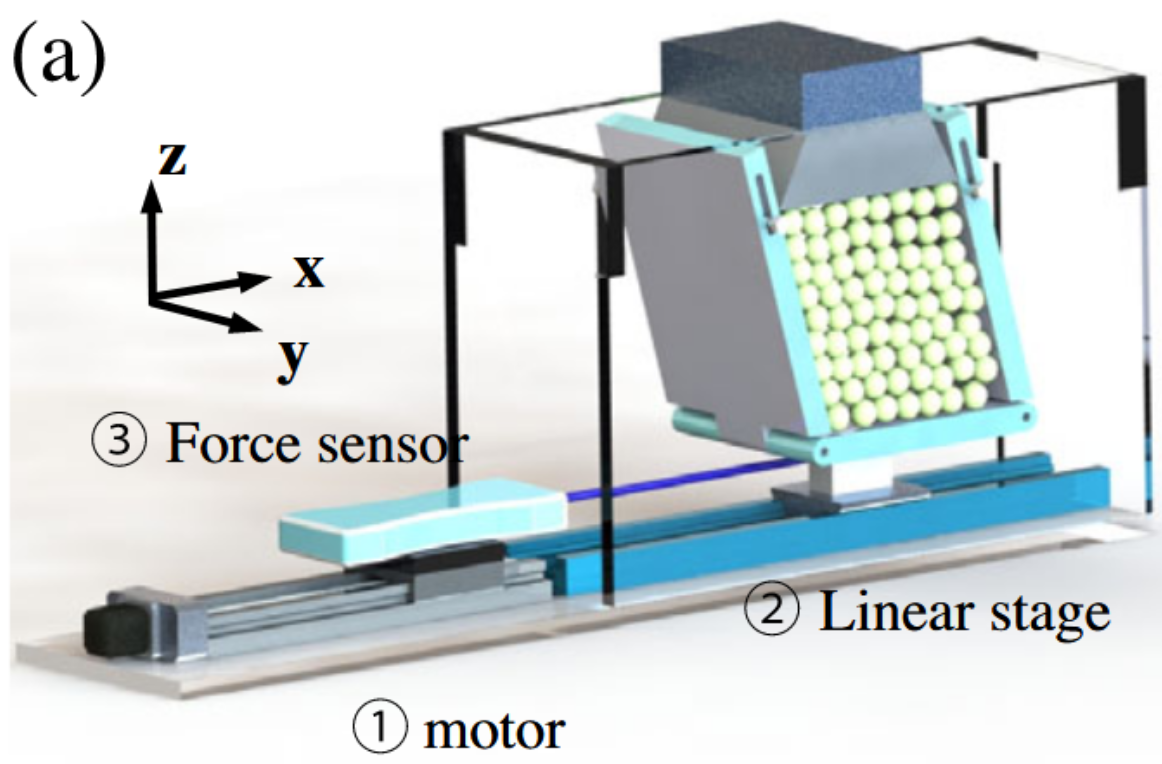
\includegraphics[height=3.5cm]{3_hloop_cycleshear_1.png}}
		\\
    \bisubcaptionbox{(a) 中颗粒介质的剪切应变 $\gamma$ 和体积分数 $\phi$、剪切应力 $F$ 的关系。}{Relationship between shear strain $\gamma$ and volume fraction $\phi$, and shear stress $F$ in granular media in (a).}
    [7cm]{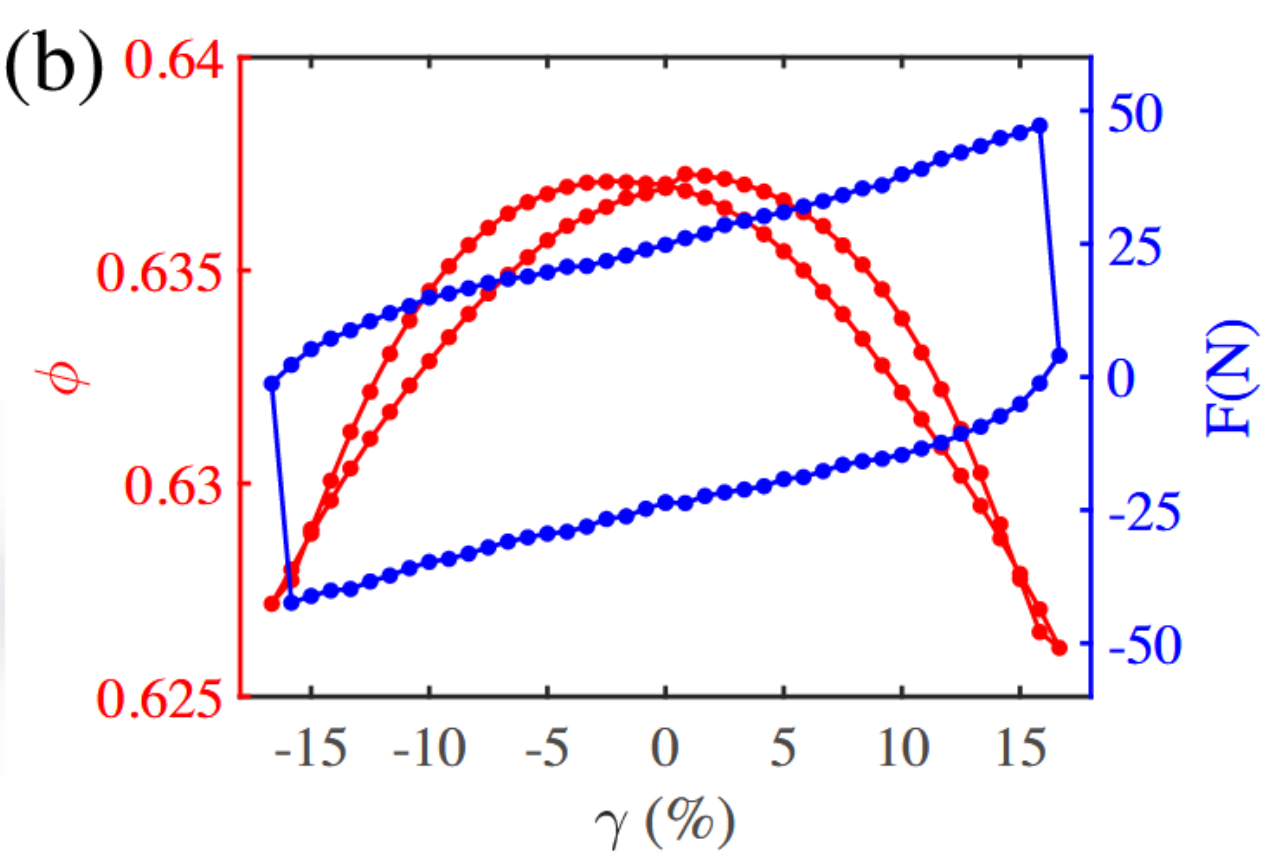
\includegraphics[height=3.5cm]{3_hloop_cycleshear_2.png}}
	\end{minipage}
	\begin{minipage}[!hbtp]{0.48\columnwidth}
		\centering
    \bisubcaptionbox{Xiaoping Jia 循环剪切实验中归一化剪切应力 $T$、剪切波(S)声速与剪切位移的演化关系。}{Evolution of normalized shear stress $T$, shear wave (S) velocity with shear displacement in Xiaoping Jia's cyclic shear experiment.}
    [7cm]{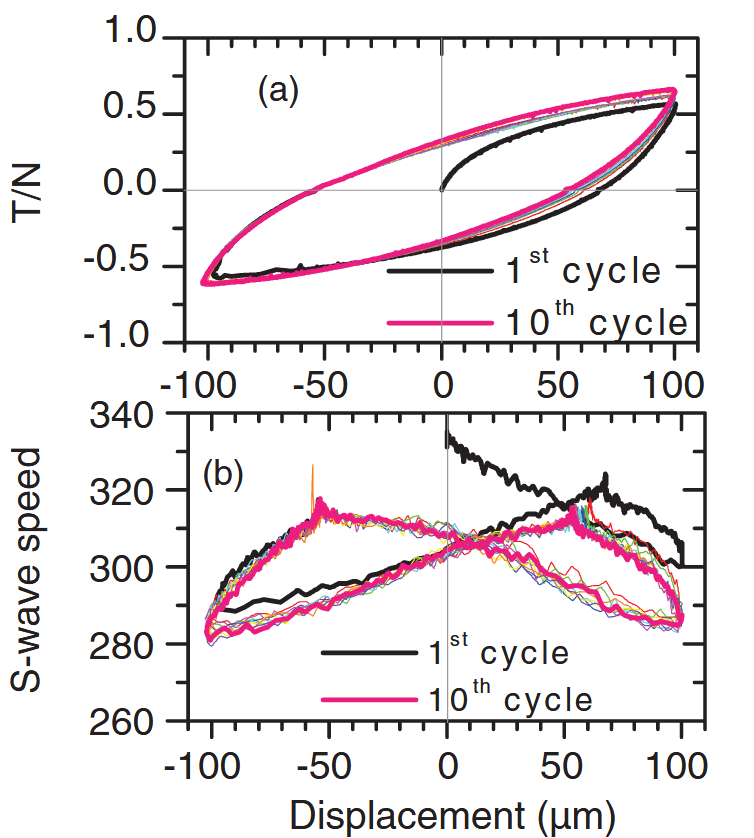
\includegraphics[height=7.5cm]{3_hloop_shearband.png}}
	\end{minipage}
	\bicaption{Yi Xing 与 Xiaoping Jia 在各自的循环剪切装置中都观察到了颗粒介质出现的滞回现象}{Hysteresis loops in granular media observed by Yi Xing and Xiaoping Jia in their respective cyclic shear apparatus.}
\end{figure}

对于颗粒间的接触力同样存在着滞回现象。我们将切向振幅视为弹性响应(Elastic,E)和耗散响应(Hysteretic,H)的线性叠加,即

\begin{equation}
  u_{t}(f_{t}) = u_{t}^{E}(f_{t}) + su_{t}^{H}(f_{t}),\quad s = \begin{cases}
    1, & f_{t} \text{ increases},\\
    -1, & f_{t} \text{ decreases}.
  \end{cases}
\end{equation}

其中 $s$ 是一个与应力过程有关的符号函数。在切向应力最大幅值 $f_{t}^{*}$ 远小于颗粒间的静摩擦阈值 $\mu f_{0}$ 时,通过 Mindlin 接触可以推导出两种响应振幅的近似表达式:

\begin{align}
  u_{t}^{E}(f_{t}) &\approx \frac{2}{3}u_{0}\left(1 + \frac{f_{t}^{*}}{6\mu f_{0}}\right)\left(\frac{f_{t}}{\mu f_{0}}\right),\label{eq:elastic_amplitude}\\
  u_{t}^{H}(f_{t}) &\approx \frac{1}{18}u_{0}\left[\left(\frac{f_{t}}{\mu f_{0}}\right)^{2} - \left(\frac{f_{t}^{*}}{\mu f_{0}}\right)^{2}\right].
\end{align}

对于式~\eqref{eq:elastic_amplitude} 进行反求导,即可得到切向接触的刚度系数:

\begin{equation}
  D_{t}^{*} = \frac{\mathrm{d}f_{t}}{\mathrm{d}u_{t}^{E}} \approx D_{t}\left(1 - \frac{f_{t}^{*}}{6\mu f_{0}}\right)
\end{equation}

因此可以推导出声速的相对变化量表达式为

\begin{align}
  \frac{\Delta V}{V}\sim \frac{\Delta D_{t}}{D_{t}} &\approx -\frac{f_{t}^{*}}{6\mu f_{0}} \sim -ku_{t}^{*},\\
  k &= \frac{2G_{g}a}{3(2-\nu_{g})\mu f_{0}}
\end{align}

由此我们推导出了两种可能的弹性软化机制。

\subsubsection{实验验证}

如果使用式~\eqref{eq:plane_wave} 来近似声信号在颗粒介质中的传播,我们可以使用类似于推导式~\eqref{eq:phase_velocity} 的方法得出衰减系数 $\alpha$ 的表达式:

\begin{equation}
  \alpha = \frac{1}{x_{2}-x_{1}}\ln{\left(\frac{S_{1}}{S_{2}}\right)}
\end{equation}

其中 $S_{1}$ 和 $S_{2}$ 分别是在 $x_{1}$ 和 $x_{2}$ 所采集信号在时域上的最大值(即去除含时系数)。但是在前面求解相速度的实验与讨论中我们已经知道,试图使用仅仅两道信号就对颗粒介质做出完整表述是几乎不可能的,需要进行系综平均以去除偶然性。因此在真正实验中,我们将使用类似于时差法测量声速的方法来测量衰减系数,即拟合声信号振幅的对数 $A$ 和传播距离/颗粒介质厚度 $L$ 的线性关系,其中斜率为 $-\alpha = \mathrm{d}[\ln{A}]/\mathrm{d}[L]$。

我们分别在应力为 9 \unit{\kilo\pascal} 和 \unit{\kilo\pascal} 的条件下,分别使用间歇激励和连续激励协议来对颗粒介质发射声信号,同时计算声速变化量、相似性参数与激励过程之间的关系。
% !TEX root = ../main.tex

\chapter{颗粒介质的剪切响应}

\section{引言}

对于颗粒间非固结的颗粒介质,其具有一定的抗剪切作用。然而颗粒间的接触及其产生的作用力很容易因为外部剪切作用导致的颗粒重排而发生变化,因此与寻常固体的应力-应变关系存在着差异。颗粒介质内部存在着不同强度的力链,其中强力链承担了介质中绝大部分的应力成分;当强力链上的颗粒成员受到外部激励而发生相对位移时,介质的应力就可能会发生较大的变化,这也是颗粒介质的奇异力学响应来源。

在第一章中我们已经提到过,等大硬球颗粒堆积存在着两种随机堆积的体积分数极限,即随机密集堆积(RCP)与随机松散堆积(RLP),这两种堆积状态的颗粒介质对于外部剪切的响应并不相同;而在密堆积中,颗粒介质也会因为所受的剪切法向应力不同而产生不同的力学响应表象。


\subsection{STZ 理论}

Shear Transformation Zone(STZ)认为,像颗粒固体这类非晶体材料在受到剪切时,会同时出现弹性形变和塑性形变,后者则是因为颗粒间发生了不可逆的相对位移。在颗粒介质受到剪切时,我们关注其中接触结构发生变化的区域。令塑性形变量为 $\varepsilon_{\text{pl}}$(pl=plastic),颗粒介质中的空隙体积为 $V_{f}$(f=free,即自由体积)。假定在剪切转变区域中存在两种不同的状态,使用 + 和 - 来对其进行表述,并引入 $n_{\mp}$ 来表示处于状态 $\mp$ 的数密度。在上述约定下,Langer 推导出了空隙体积变化率方程\cite{PhysRevE.64.011504}:

\begin{equation}
  \dot{V_{f}} = -E_{1}\cdot{\ee}^{-\frac{V_{1}}{V_{f}}} + A_{V}|\sigma\dot{\varepsilon}_{\text{pl}}|,
\end{equation}

其中 $E_{1}$、$A_{V}$ 是常数,$V_{1}$ 表示的是受剪切区域刚发生变化时的自由体积大小(也被称作临界自由体积),$\sigma$ 表示介质所受的偏应力。$\varepsilon_{\text{pl}}$ 定义如上,且存在关系

\begin{align}
  \dot{\varepsilon}_{\text{pl}} = E_{0}{\ee}^{-\frac{V_{0}}{V_{f}}}\left[\Lambda\sinh{(\sigma)} - \Delta\cosh{(\sigma)}\right],\\
  \Lambda = \frac{n_{-} + n_{+}}{n_{\infty}},\quad\Delta = \frac{n_{-} - n_{+}}{n_{\infty}}.
\end{align}

其中 $n_{\infty}$ 是 $(n_{-} + n_{+})$ 在稳定平衡态下的值。对于 $\Lambda$ 和 $\Delta$,其行为被描述为

\begin{align}
  \dot{\Delta} &= \frac{1}{\varepsilon_{0}}\left(\dot{\varepsilon}_{\text{pl}} - \gamma|\sigma\dot{\varepsilon}_{\text{pl}}|\Delta\right),\\
  \dot{\Lambda} &= \frac{\gamma}{\varepsilon_{0}}\left|\sigma\dot{\varepsilon}_{\text{pl}}\right|(1-\Lambda)
\end{align}

使用 STZ 理论,可以描述颗粒介质在受剪切时出现的蠕变和滞滑现象。

\section{实验装置}

目前剪切装置和声学装置的耦合尚不成熟,因此只简要介绍有关于剪切装置的部分。图~\ref{fig:apparatus_2} 展示了剪切实验中的各部件。

\begin{figure}[!htp]
    \centering
    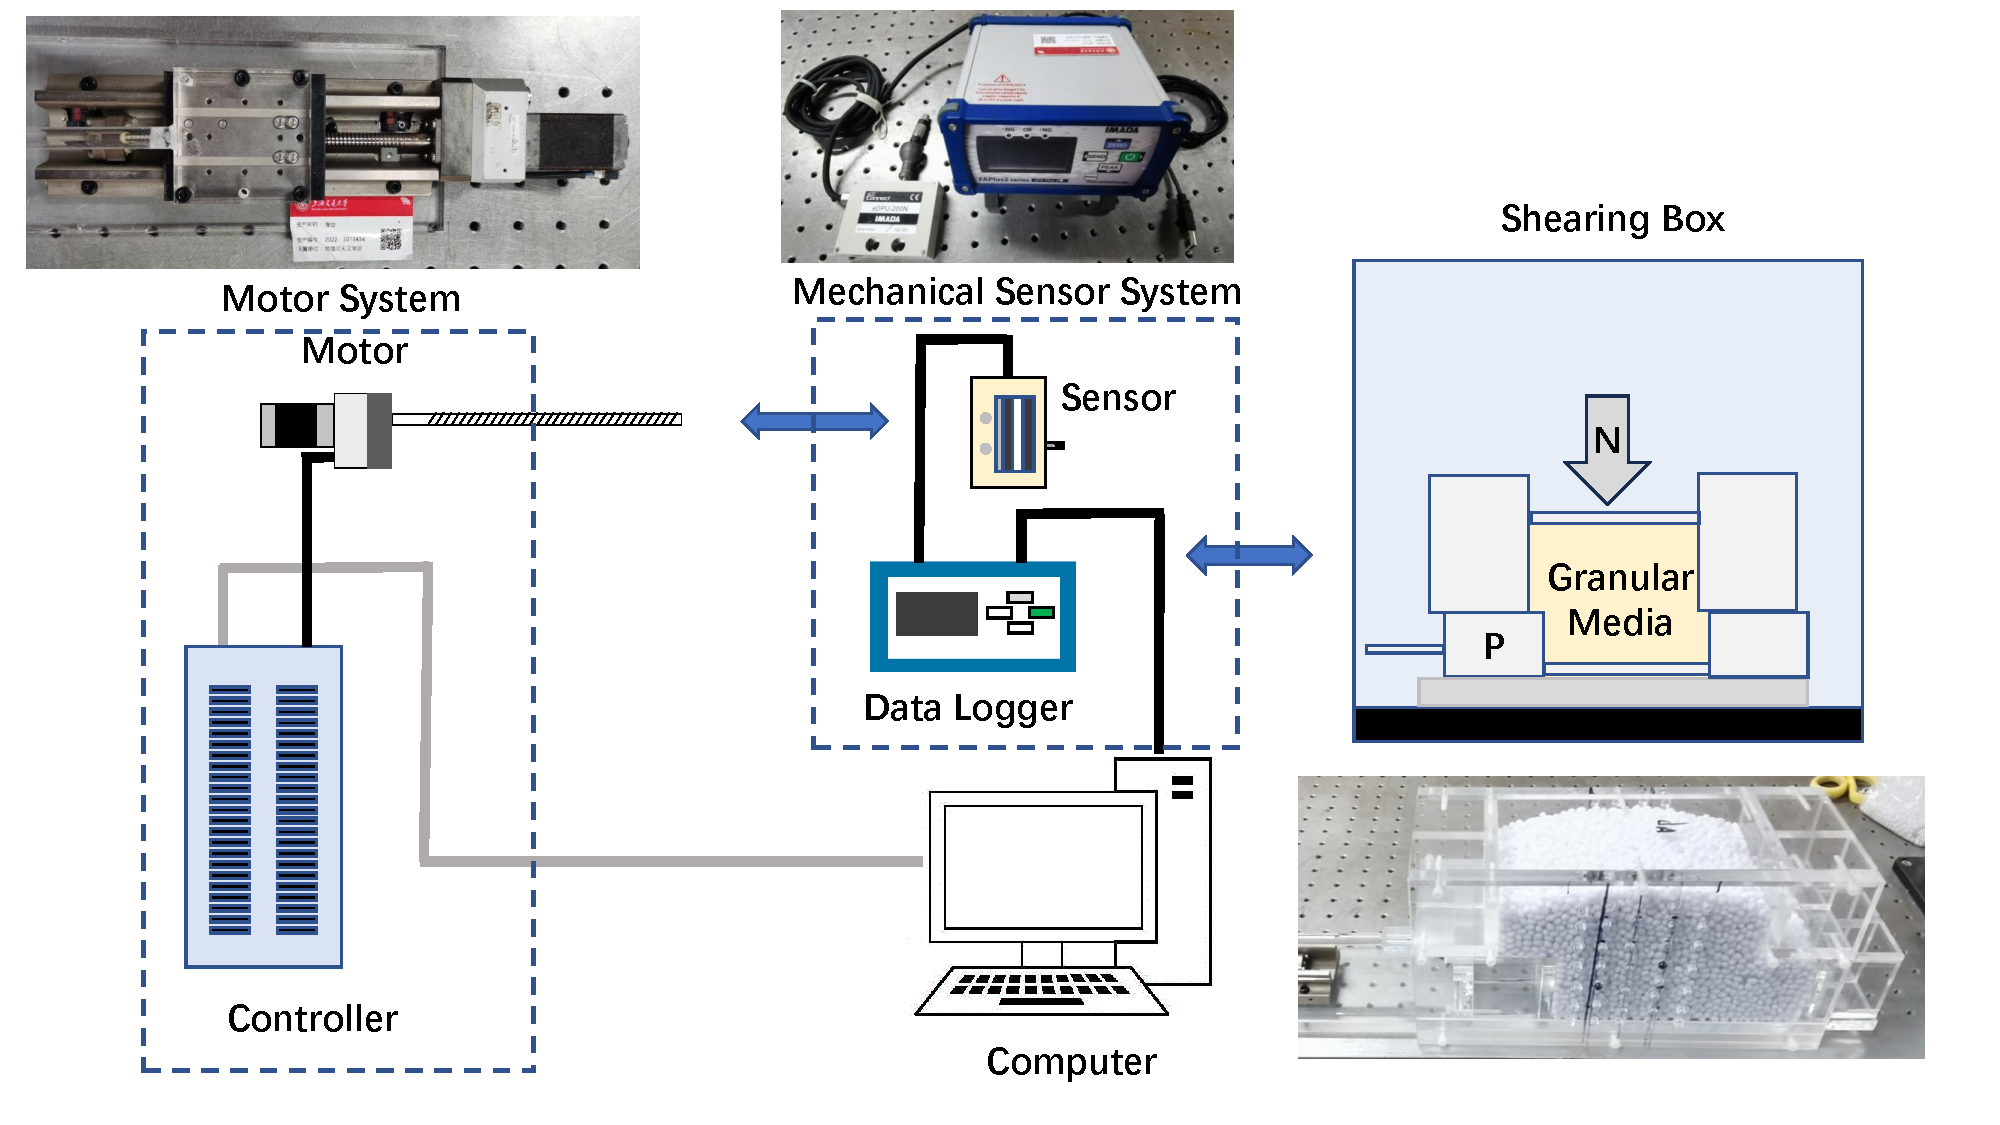
\includegraphics[height=8.5cm]{figures/4_apparatus.pdf}
    \caption{剪切装置与数据收集系统示意图}
    %{Schematic diagram of the shearing apparatus and data collection system}
    \label{fig:apparatus_2}
  \end{figure}

接下来我们来介绍各部件的主要功能:

\begin{enumerate}
    \item 骏河步进电机。通过连杆与剪切盒的活塞部分固定连接,从而推动其进行对颗粒介质的剪切。电机通过 D214-2-2ek 信号线连接至控制器,控制器通过 USB 信道连接至计算机。计算机通过 DSCONTROL-WIN 软件来对电机进行控制,可以控制电机的运动方式为连续/步进,电机旋转方向和速度等参数。
    \item IMADA 力学传感系统。由 Sensor 和 Data Logger 两部分组成,Sensor 通过信号线将感受的力大小传递至 Data Logger;后者通过 USB 信道将数据实时传递至计算机,通过 Force Recorder 软件读取数据,力学传感器的最高采集频率为 2000 \unit{\hertz},力的分辨率则是 0.1 \unit{\newton}。在所需数据记录完毕后,即可通过 .csv 格式导出以供数据分析。
    \item 剪切盒。材质和单轴应力容器所使用的材质一样,是由亚克力板制作的,原本用于 X 光辐照探测剪切带。在未剪切时,其内部容积为 $18\times 10\times 12$ $\unit{\centi\meter}^{3}$ 的立方体,受电机控制的横截面积为 $10\times 6$ $\unit{\centi\meter}^{2}$ 的活塞带动固连的底板进行推动,而所推动的活塞截面的高度小于颗粒介质的高度而对颗粒介质有剪切作用。由于剪切盒的活塞在运动方向上存在长度上限,为了避免颗粒漏出剪切盒的剪切应变也存在上限。剪切盒的封顶板可以拆下而替换为施加应力的活塞板,从而检测不同堆积方式的颗粒介质的力学响应机制。
\end{enumerate}

\section{应力-应变曲线}

\subsection{RCP 与 RLP 的剪切响应差异}

我们使用同一剪切装置,在未施加应力与施加应力 P = 3.97 \unit{\kilo\pascal} 下分别测定 6 \unit{\milli\meter} ABS 球所组成的颗粒介质的应力-应变曲线。为了充分展现颗粒介质的滞滑特性,我们在实验时设定的剪切速率极低;在 DSCONTROL-WIN 软件上设定的剪切速率为 20 \unit{pps},对应于现实世界的剪切速度约为 $60\sim 70$ \unit{\micro\meter}/\unit{\second}。图~\ref{fig:shearstress} 展示了以上两种堆积在相同剪切速率下的剪切应力-应变曲线,其中定义域分别为剪切位移和时间。

\begin{figure}[htbp]
	\centering
	\subcaptionbox{随机松散堆积的剪切应力-应变曲线}%
                  %{Shear stress-strain curves for random loose packing}%
                  [15cm]{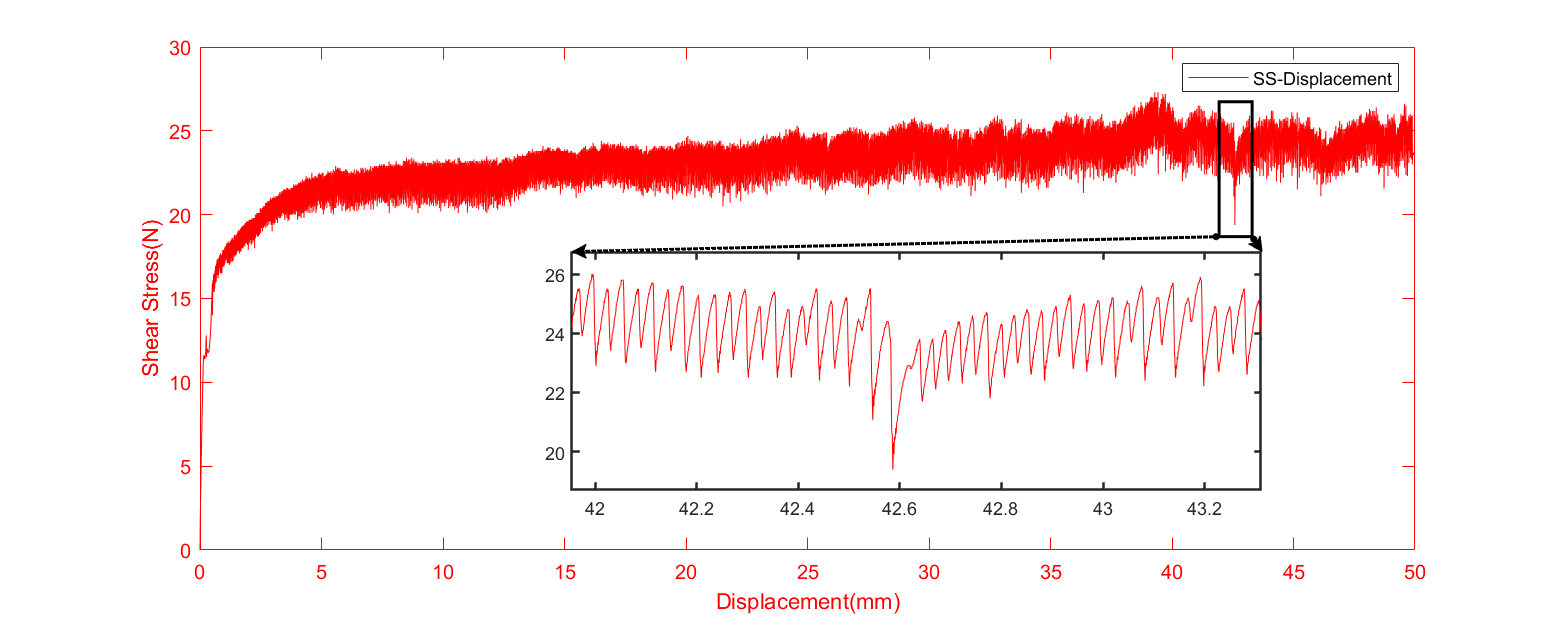
\includegraphics[width=1\linewidth]{4_shearstress_displacement.png}}\\
  \subcaptionbox{随机密集堆积的剪切应力时域曲线}%
                  %{Shear stress in time domain for random close packing}%
                  [15cm]{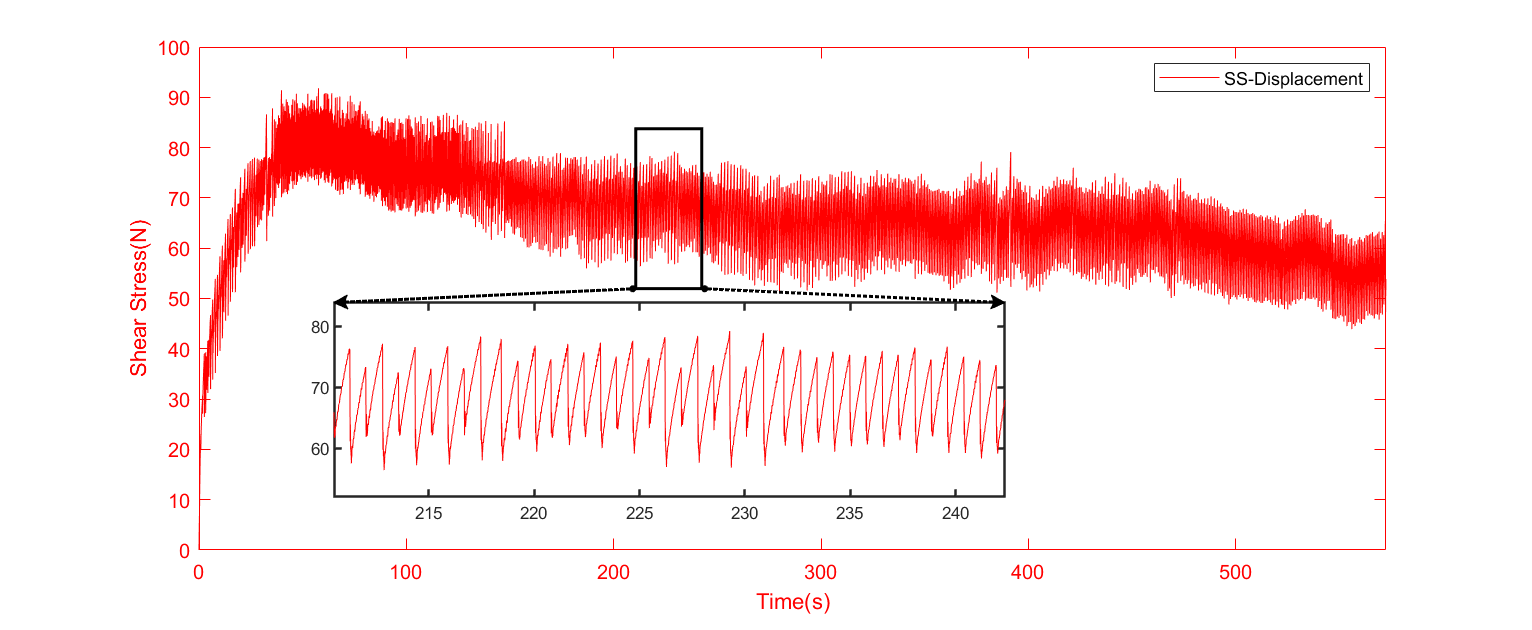
\includegraphics[width=1\linewidth]{4_shearstress_time.png}}
  \caption{RLP 与 RCP 在剪切速率为 20 pps 下的力学响应曲线}%{Mechanical response curves of RLP and RCP at shear rate of 20 pps}
  \label{fig:shearstress}
\end{figure}

\subsection{蠕变与滞滑}

在 RCP 中得到的应力曲线更接近于传统的固体材料,即分为弹性区、屈服区(yielding state)和临界区(critical state)。

\begin{itemize}
  \item 弹性区。在剪切位移较小时,大部分颗粒位置几乎不变,而只是存在着较小程度的挤压和摩擦,这种接近线性的应力-应变关系和弹性行为相似,即产生蠕变现象;
  \item 屈服区。当剪切位移增大到一定程度时,即颗粒间的相互摩擦开始接近静摩擦阈值,颗粒开始产生相对滑动、重排,并且这种过程是不可逆的。应力的最高点即为颗粒介质的屈服强度。从放大图像观察可知,出现了剪切应力的反复积累提升、骤降的现象,这种过程伴随着频繁的力链断裂和重构,即滞滑。
  \item 临界区。在剪切位移进一步增大时,此时颗粒介质展现出可被类比于固-液相变的性质,即颗粒介质在外部剪切的激励下出现了流动的现象。
\end{itemize}

我们可以按照应力降(Shear Stress Drop,SSD)的大小来对滞滑事件进行粗分类。类比于环形剪切相关实验中的方法,我们按照应力降的幅值将滞滑事件分为三类:微滞滑(micro-,$\text{SSD}<0.2$ \unit{\newton})、小滞滑(minor-,0.2 \unit{\newton}$<\text{SSD}<0.4$ \unit{\newton})和主滞滑(major-,在地震学也被称作 failure,$\text{SSD}>0.4$ \unit{\newton})。我们统计了微滞滑事件的数量以及其在最近主滞滑事件前的时间间隔,从而得到了通过微滞滑事件计数来预测可能的滞滑失效事件的事件。我们对微滞滑的发生数量进行了对数处理后绘制了图像~\ref{fig:preceding_interval}。其解读方式是,在发生了一次主滞滑事件后,对微滞滑进行计数,若已经发生了 $N$ 次,则下一次主滞滑可能发生的时间间隔为 $T(log{(N)})$ \unit{s}。

\begin{figure}[!htp]
  \centering
  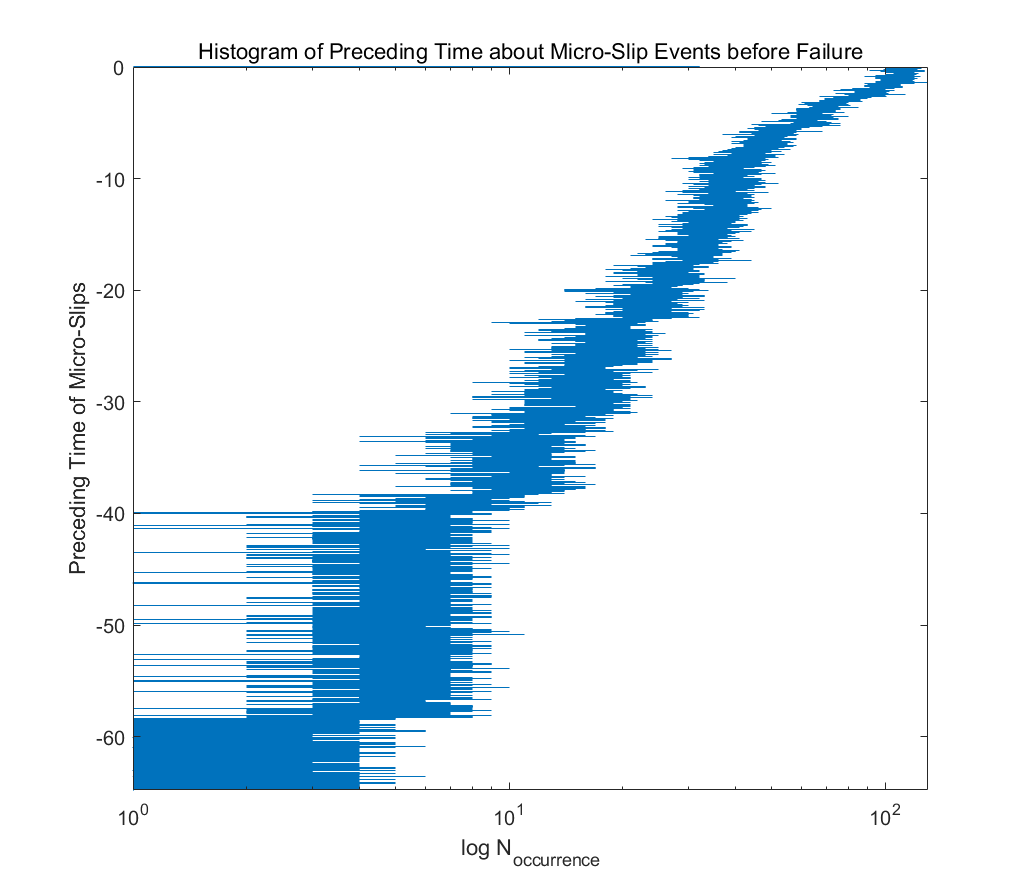
\includegraphics[height=10cm]{figures/4_preceding_interval.png}
  \caption{微滞滑数量及其最近邻失效前时间间隔的直方图}
  %{Hsitogram of preceding interval of micro-slip events before the neighboring failure}
  \label{fig:preceding_interval}
\end{figure}

可以观察到其大致从原点引出了一条直线,而在原点附近出现了拐点,推测是因为力学传感器本身会出现一定的分辨率程度的波动($\sim$ 0.1 \unit{\newton}),使得微滞滑的计数偏多。在未来引入多通道采集卡,从而通过声学手段辅助分析剪切过程中的滞滑事件,将有助于得到更理想的图像结果。

\section{本章小结}

本章检测了在同一剪切速率下,无法向应力的 RLP 与有法向应力的 RCP 的应力应变的区别,并且通过统计的方法对颗粒介质在受剪切过程中的滞滑事件进行现象学分析,从而得到了预测主滞滑(即滞滑失效)的可能时间,有助于应用在地震学领域进行地震预测。
% !TeX root = ../main.tex

% !TEX root = ../main.tex

\chapter{全文总结}

颗粒介质中的超声信号一般可分为相干首波和散射尾波,小振幅时具有探测作用,有限振幅时则具有泵浦作用。对于相干波部分,我们通过飞行时间法和频散能量图法测定了颗粒介质中的声速,并且检查了声速和颗粒介质应力之间的指数关系,分析了其与等效介质理论之间差异的可能原因;观察到了首波的展宽现象,通过归一化宽度对其进行表述,其在不同厚度的颗粒介质中的值与通过一维随机层理论导出的预测符合较好。对散射波部分,我们通过截断级数拟合功率时域图,计算得到平均自由程和品质因子,从而检验了扩散行为近似导出的辐射传递方程的符合较好;通过增大激励信号的幅值,检验了颗粒介质中的非线性波激发现象,并且通过相似性参数和声速观察到了声波对于颗粒介质产生的不可逆泵浦作用。在对颗粒介质进行剪切时,观察到了 RLP 和 RCP 的不同应力-应变曲线,并且通过滞滑事件计数进行了滞滑失效统计预测的现象学分析。而利用相似性参数检测颗粒介质中的剪切带和监测受剪切过程的声发射事件有待后续研究。

%TC:ignore

% 参考文献
\printbibliography[heading=bibintoc]

% 附录
\appendix

% 附录中图表不加入索引
\captionsetup{list=no}

% 附录内容
%\input{contents/app_maxwell_equations}
%% !TEX root = ../main.tex

\chapter{绘制流程图}

图~\ref{fig:flow_chart} 是一张流程图示意。使用 \pkg{tikz} 环境,搭配四种预定义节
点(\verb|startstop|、\verb|process|、\verb|decision| 和 \verb|io|),容易地绘制出流程图。

\begin{figure}[!htp]
  \centering
  \input{figures/flow_chart.tex}
  \bicaption{绘制流程图效果}{Flow chart}
  \label{fig:flow_chart}
\end{figure}


% 结尾部分
\backmatter

% 用于盲审的论文需隐去致谢、发表论文、科研成果、简历

% 致谢
% !TEX root = ../main.tex

\begin{acknowledgements}
  
\end{acknowledgements}


% 发表论文及科研成果
% 盲审论文中,发表论文及科研成果等仅以第几作者注明即可,不要出现作者或他人姓名
% !TEX root = ../main.tex

\begin{achievements}

% \subsection*{学术论文}

% \begin{bibliolist}{00}
%   \item Chen H, Chan C~T. Acoustic cloaking in three dimensions using acoustic metamaterials[J]. Applied Physics Letters, 2007, 91:183518.
%   \item Chen H, Wu B~I, Zhang B, et al. Electromagnetic Wave Interactions with a Metamaterial Cloak[J]. Physical Review Letters, 2007, 99(6):63903.
% \end{bibliolist}

% \begin{bibliolist*}{00}
%   \item 第一作者. 中文核心期刊论文, 2007.
%   \item 第一作者. EI 国际会议论文, 2006.
% \end{bibliolist*}

% \subsection*{专利}

% \begin{bibliolist}{00}
%   \item 第一发明人, “永动机”, 专利申请号202510149890.0.
% \end{bibliolist}

% \begin{bibliolist*}{00}
%   \item 第一发明人, “永动机”, 专利申请号XXXXXXXXXXXX.X.
% \end{bibliolist*}

\end{achievements}


% 简历
% !TEX root = ../main.tex

\begin{resume}
  \subsection*{基本情况}
    何翼成,2002 年 2 月生于重庆市大足区。

  \subsection*{教育背景}
  \begin{itemize}
    \item 2020 年 9 月至今,上海交通大学,本科生,物理学专业
  \end{itemize}

  \subsection*{研究兴趣}
    颗粒介质物理

  \subsection*{联系方式}
  \begin{itemize}
    \item 地址: 上海市闵行区东川路 800 号,200240
    \item E-mail: \email{heyicheng@sjtu.edu.cn}
  \end{itemize}
\end{resume}


% 学士学位论文要求在最后有一个大摘要,单独编页码
% !TEX root = ../main.tex
%

\begin{digest}

\end{digest}


%TC:endignore

\end{document}
